% $Id:$

\section{\label{sec:stosoft}Storage Manager Software}  %Editor: Harry

\subsection{Storage Manager Functions}

The primary function of the Storage Manager (SM) is to collect (event) data from
each Event Filter Farm HLT (High Level Trigger) process, and store them in files
for Tier-0 to pickup and process.
The event data files are written to a set of output streams according to
the event trigger bits and the SM configuration information.

The Storage Manager also acts as an event server, and a DQM (Data Quality
Monitoring)  data server for consumer clients. The DQM data is produced in the
Filter Farm HLT processes which has access to the full L1
trigger rate of events before the HLT. The consumers analyze event data
or DQM data and are mainly used for monitoring the data, or possibly for calibration
and alignment.

The DQM data or monitoring elements are mainly histograms filled with data for a particular
period of time, nominally one luminosity section (LS) or about 93 seconds
during normal running. Each specific histogram is produced in each HLT process
but contain different events for a given LS. So for each LS, all these
histograms need to be added together. Besides gathering the histograms
from each HLT process together in the Storage Manager, the SM has the additional 
function of adding up histograms of the same type from each HLT process.
The summed histograms are then written out and passed to the DQM system.

These functions of the Storage Manager are represented schematically
in Fig.~\ref{fig:schematic_simple}.

\begin{figure}[hbtp]
  \begin{center}
    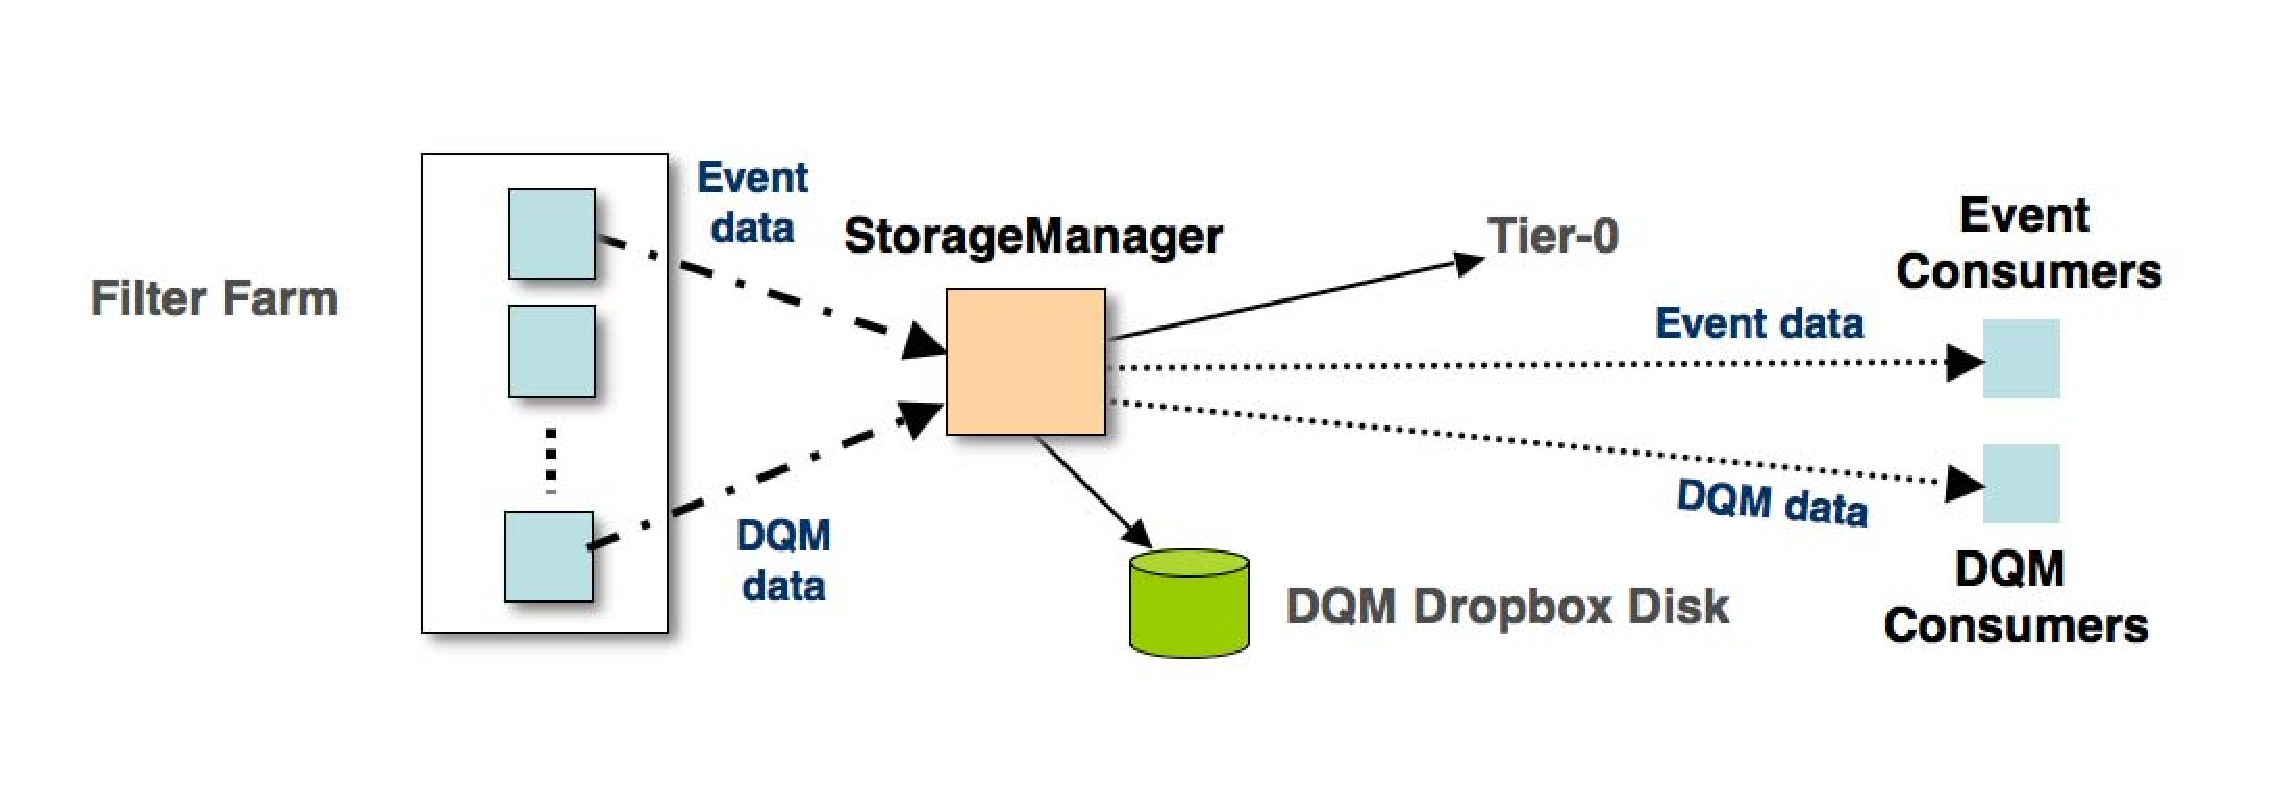
\includegraphics[width=5.5in]{Software/schematic_simple}
    \caption{Functional schematic.}
    \label{fig:schematic_simple}
  \end{center}
\end{figure}

\subsubsection{Software Responsibilities}

The Storage Manager project software task has well defined  responsibilities. The
functions of the code needed are listed below. 

\begin{itemize}
\item Serialize data into a byte stream for network transfer.
\item Create and maintain the serialized data format.
\item Provide input modules to deserialize and reform the data for the framework.
\item Receive data from all HLT processes in the Filter Farm.
\item Output event data in streams based on trigger bits.
\item Communicate and interact with Tier-0 for data transmission to Tier-0.
\item Serve event data and DQM data to consumers.
\item Receive DQM data, sum histograms and output to DQM Disks.
\end{itemize}

Much of the Storage Manager software is well integrated within the standard
CMS offline framework. In fact the base classes for the serialized data input
source ad serialized data output modules are provided and maintained by the
CMS framework group.

\subsubsection{Requirements and Dependencies}

The Storage Manager runs in the CMS online system which is implemented within
the XDAQ framework. The Storage Manager application must be a XDAQ application
operating within the CMS DAQ and configured, controlled, and monitored by the
CMS Run Control.

The Storage Manager must be able to handle the required data rates and the
primary event data collection and output must not be compromised by the other
functions of the Storage Manager.

The event data and DQM data consumers must be able to receive the data using a
standard CMS EDM offline framework job, or a CMS XDAQ consumer application.
There is currently no requirement for remote consumers, {\em i.e.} ones that operate
from outside of the experimental private network.

The strategy of the Storage Manager group is to reuse as much of the code in
the CMS offline framework, the CMS DAQ, and the DQM framework. This
integration means that the SM code is highly dependent on these three 
subsystems.

\flushleft{\em Handling of Events with Different Data Products}

The HLT process will produce data where events can have different data products. An example
use case is the production of the following streams:

\begin{itemize}
\item Physics stream saving all main products (data branches)
\item Calibration stream saving only a few data products; high rate
\item Debug physics stream saving all main products and in addition many intermediate 
data products for debugging; low rate
\item Exception stream where HLT modules have failed; very low rate
\item Auto-accept (small fraction of all events passing L1); low rate
\end{itemize}

Separately there is an Error Stream that does not actually go through the HLT. This 
Error stream is for events that cause a HLT process to die or time out. These events 
go directly from the Resource Broker to the Storage Manager.

Due to a limitation of the offline software framework, all events in a particular output
stream file must have exactly the same set of data products. Events with different
data products cannot be mixed into the same file.


\subsection{Architecture}

The approximately 640 Filter Farm nodes will be split into 8~(or multiple of 8) separate
slices or subfarms. Each subfarm will have its own Storage Manager application
instance as illustrated in Fig.~\ref{fig:SM_architecture_base}. A separate XDAQ 
SM Proxy Server application collects events at a low rate from the
Storage Managers of each subfarm to serve to event consumers. The SM Proxy
Server application also collects DQM data and sums the DQM histograms before
outputing these summed DQM data to the DQM disks. All Storage Manager
instances and the  SM Proxy Server
application sits inside the CMS DAQ private network.

Each Storage Manager application also has event data and DQM data server
functions, however in normal running the Storage Managers will be isolated from
all consumers by the SM Proxy Server.

\begin{figure}[hbtp]
  \begin{center}
    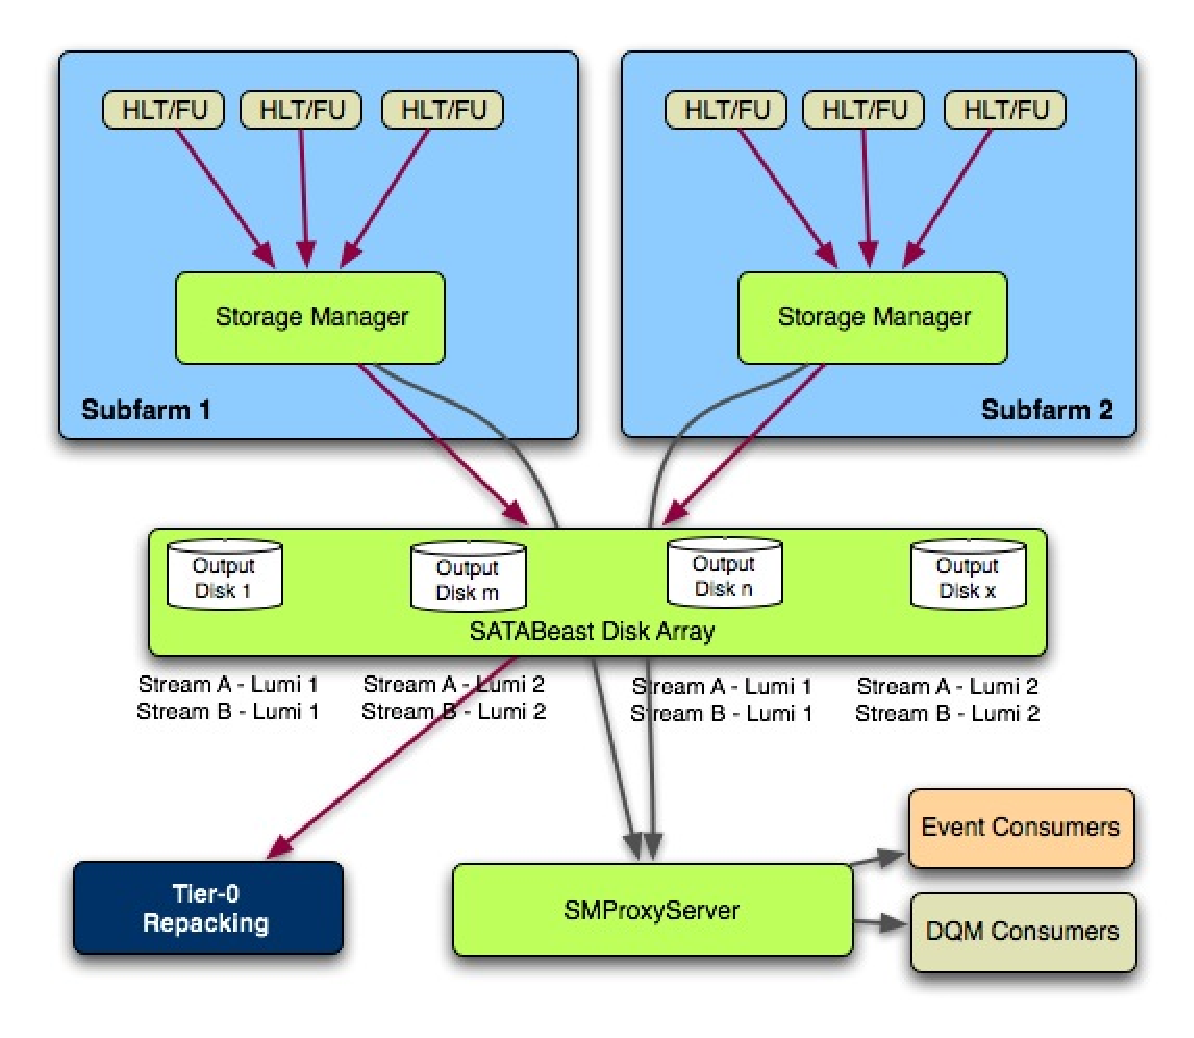
\includegraphics[width=4.5in]{Software/SM_architecture_base}
    \caption{Architecture with subfarms.}
    \label{fig:SM_architecture_base}
  \end{center}
\end{figure}

\subsubsection{Routing of Events in the Storage Manager}

It was decided to implement multiple output streams with different data products by using
multiple HLT output modules, where each output module gives events with a certain
data product selection.
The HLT output module, Resource Broker, and Storage Manager software need to handle 
the following issues:

\begin{itemize}
\item HLT output modules are able to drop products independently (no assumption 
that one output module will contain the whole superset of data products).
\item An event can satisfy the selection for multiple output modules, and thus need 
to go to multiple streams in the Storage Manager with the correct data products.
\item The Storage Manager must write streamer files that are readable and can be 
converted to Root files irrespective of what data products are kept for the stream (file).
\end{itemize}

The data for each HLT output module is tagged with the output module identifier,
 the SM uses this output module id as well as the event trigger bits to direct events to the
 correct output stream file. The HLT and SM configuration are thus coupled and must be 
 correctly setup to route events to the correct output streams.


\subsection{Software Components}

In this section we describe each of the software components that form the
Storage Manager software project. These are represented by the circles/ovals in
Fig.~\ref{fig:schematic_wproxy}. The hardware view from 
Fig.~\ref{fig:system} is used in Fig.~\ref{fig:sm_hardware_wsoftware}
to illustrate where the software components run.

\begin{figure}[hbtp]
  \begin{center}
    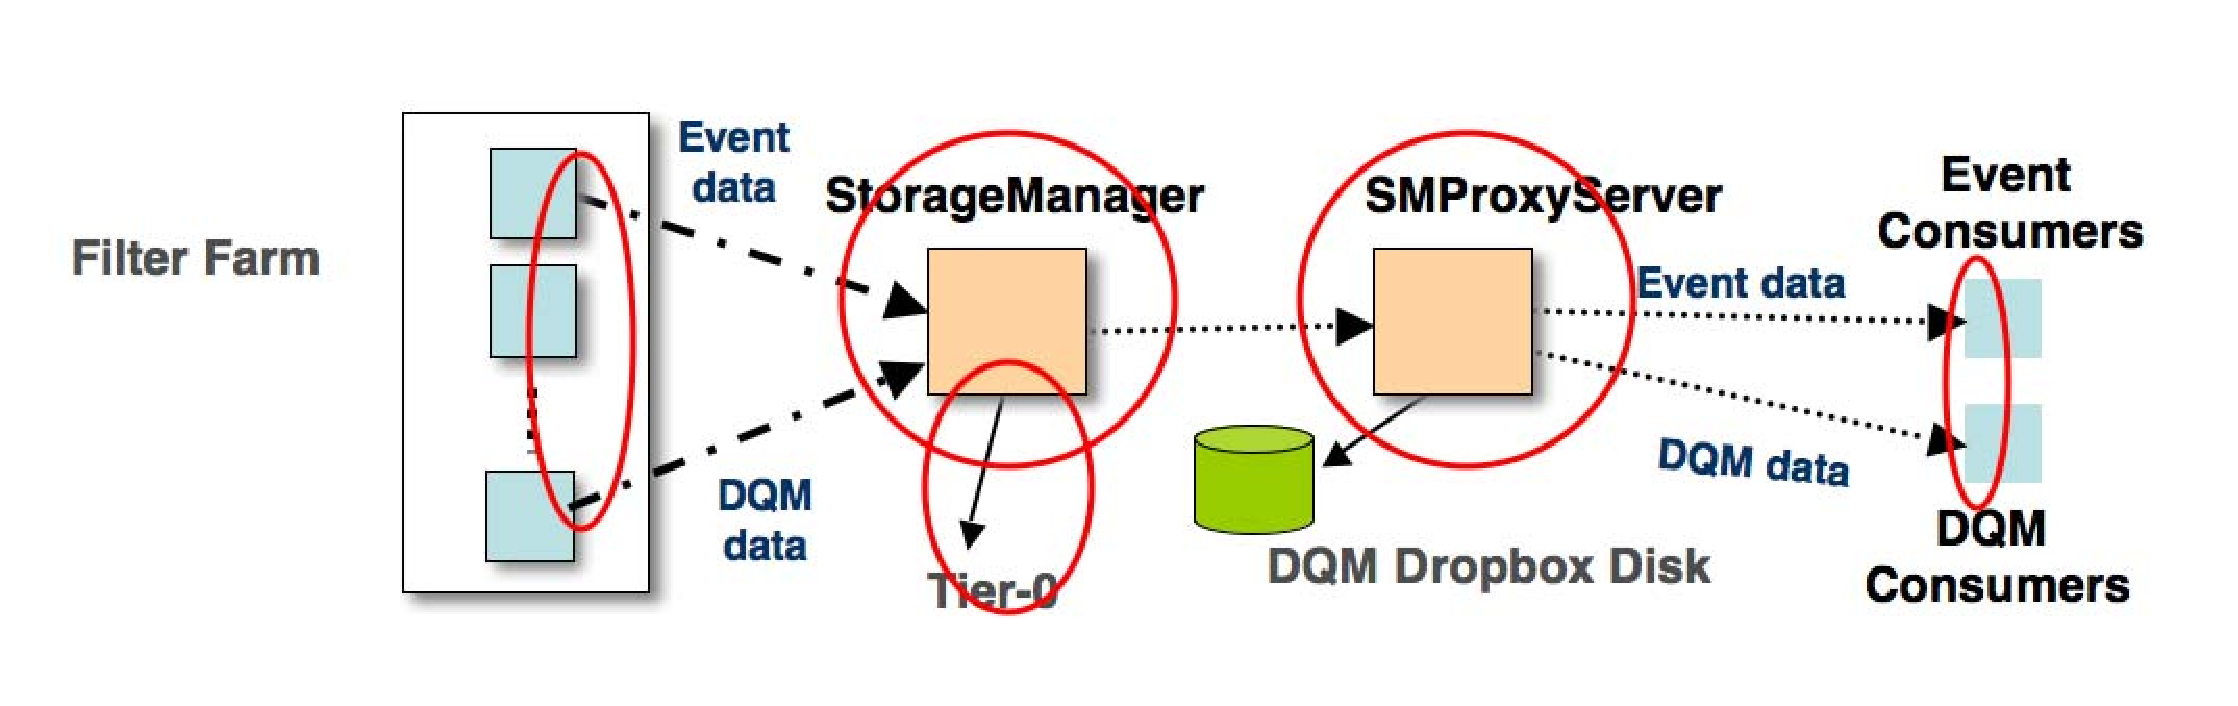
\includegraphics[width=5.5in]{Software/schematic_wproxy}
    \caption{Functional schematic with subfarms.}
    \label{fig:schematic_wproxy}
  \end{center}
\end{figure}

\begin{figure}[hbtp]
  \begin{center}
    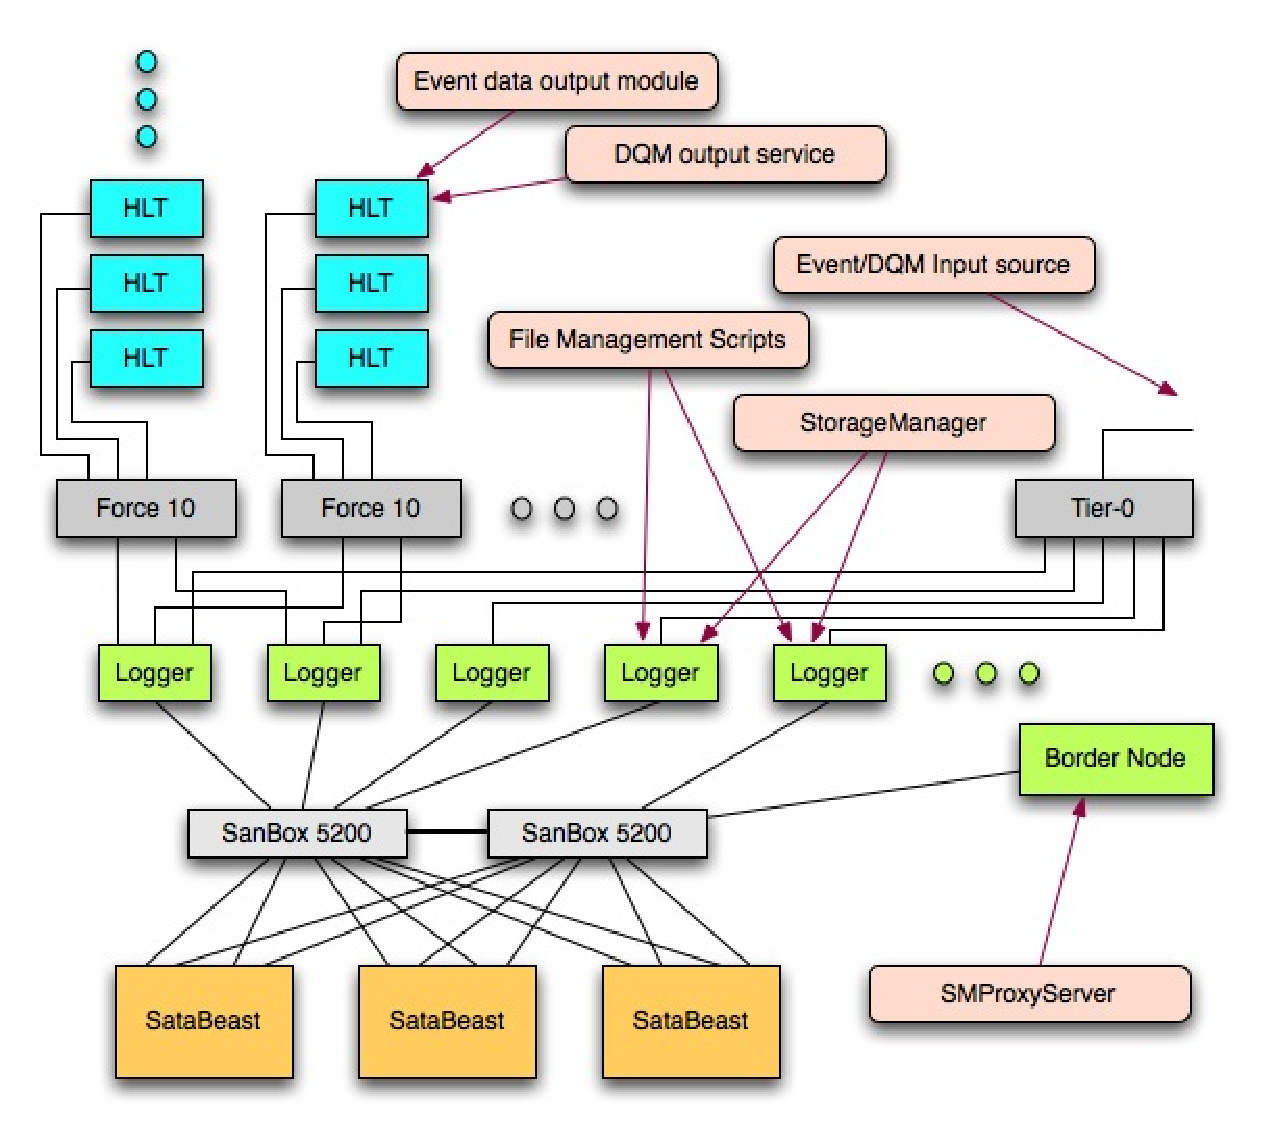
\includegraphics[width=4.5in]{Software/sm_hardware}
    \caption{Hardware view showing where the software components run.}
    \label{fig:sm_hardware_wsoftware}
  \end{center}
\end{figure}

\subsubsection{Output and Input Modules}

The Storage Manager group provides the CMSSW framework (FW) 
output module for the HLT process. In
the output module the event data are serialized into a ``blob'' of bytes for
transfer over the network to the Storage Manager. The actual transfer is
done by the Resource Broker running the on the HLT Filter Farm node via
the I2O facility in XDAQ. This is illustrated in Fig.~\ref{fig:ps_fudesign}.
The ``data blob'' is written to shared memory which is managed by the
resource broker.

\begin{figure}[hbtp]
  \begin{center}
    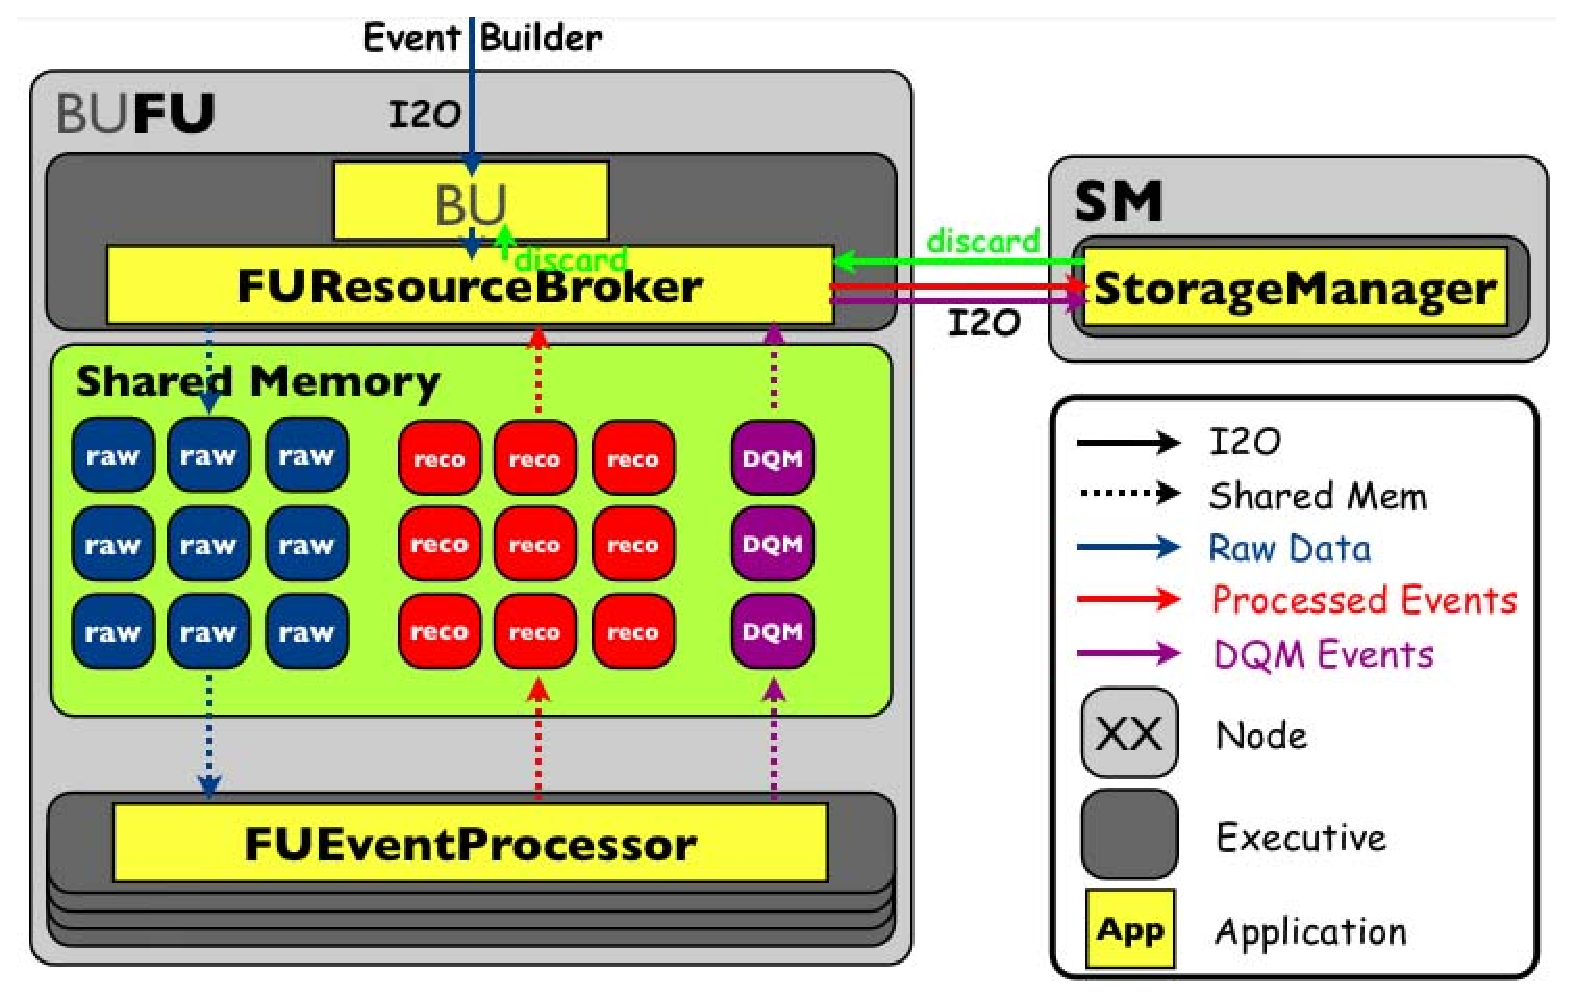
\includegraphics[width=5.5in]{Software/ps_fudesign}
    \caption{Schematic showing the mechanism for data transfer between the
HLT process (FUEventProcessor) and the Storage Manager.}
    \label{fig:ps_fudesign}
  \end{center}
\end{figure}

Since the maximum size of I2O frames is 256~KB, and the actual I2O frame
size used in the CMS online is smaller (64~KB), the resource broker 
splits the data for each event into as many fragments as needed, wraps each fragment with
appropriate I2O headers and sends them to the Storage Manager. The code for
doing the split of the ``data blob'' was initially provided by the Storage Manager
group though it now resides in the Resource Broker software package and
maintained by the CMS DAQ group.

The output module is a plugin module of the CMS offline framework and can be
used in either a standard CMS offline job (using cmsRun), or within the online
HLT process. The online HLT process uses an instance of CMS offline framework
event processor running in an asynchronous mode, and basically has the same
features as an offline event processor except its execution can be controlled
by the CMS Run Control.

The output module inherits from an output module class provided by the CMS
offline framework group, thus the main maintenance load is with the data
serialization. The output module is actually a templated class and another
output module using the same template is also maintained that writes out
streamer files instead of to shared memory. This additional streamer file
output module is used internally for testing purposes.

The Storage Manager group provides a DQM output service plugin module.
The output service uses the standard offline framework hooks for its
processing schedule, and the main function is to serialize the
DQM data and write to shared memory.

The Storage Manager group also provides two input source plugin modules,
one for streamer file input and one for network input. Both inherit from
a base input source provided and maintained by the CMS framework group.
The streamer file input source is used primarily by the Tier-0 group
but is also used internally for testing purposes. The network streamer input
module is used for event data consumers for online monitoring.
These input sources does the deserialization needed to convert the serialized
data back into CMS framework event objects.

The network input source used by the online consumers use cURL to
interact with the HTTP server of the Storage Manager application, and uses a 
HTTP GET command to receive data in a binary stream.

These input sources are not used inside the Storage Manager itself.
No deserialization of the event data is done in the Storage Manager, and it does not
use the CMS framework event processor. 
Deserialization of DQM histogram data may take place in the Storage Manager
so that the same histogram from multiple HLT processes can be summed before
sending to the SM Proxy Server.
Details of the Storage Manager and SM Proxy Server input
and processing is given below in the respective application description sections.

\subsubsection{Serialization and Deserialization}

A serialized data format was created for the serialized data. Originally this
format was to be a completely temporary format used only for the network
transfer of event data to the Storage Manager. The Storage Manager would then
write out standard CMS ROOT files. During the testing of the first prototype
of the Storage Manager we found that the deserialization performance was too
poor to write out standard CMS ROOT files. Instead in the second prototype
we wrote out flat binary files, called streamer data files, these are basically
the concatenation of each of the event serialized data messages
sent over the network.

\begin{figure}[hbtp]
  \begin{center}
    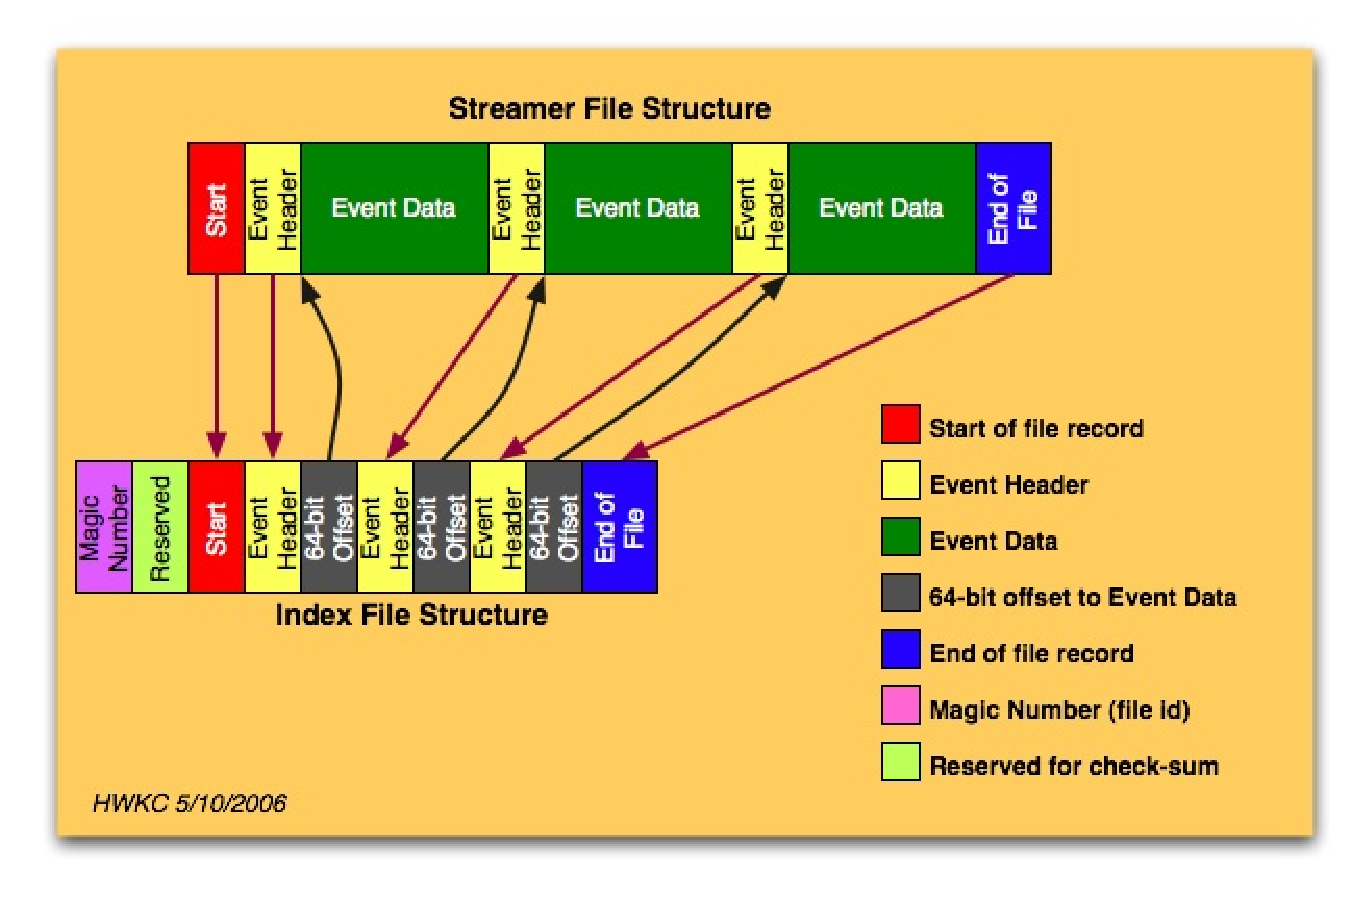
\includegraphics[width=5.5in]{Software/sm_messages1}
    \caption{Schematic showing the format of Streamer files and index files.}
    \label{fig:sm_messages1}
  \end{center}
\end{figure}

The streamer file format is illustrated in Fig.~\ref{fig:sm_messages1}. The file
consists of a start of file record, and an event record for each event, and
an end of file record is placed at the end of the streamer file. The event
record consists of an event header and the event data.

The actual formats of the start of file record, the event header and data, and the
end of file record are given schematically in Fig.~\ref{fig:sm_mess_structure}.
The formats of the start of file record, and the event record are exactly the
same as the format of messages used to transfer data from the HLT process to the
Storage Manager. This has the advantage of having less code for the Storage
Manger group to maintain.

\begin{figure}[hbtp]
  \begin{center}
    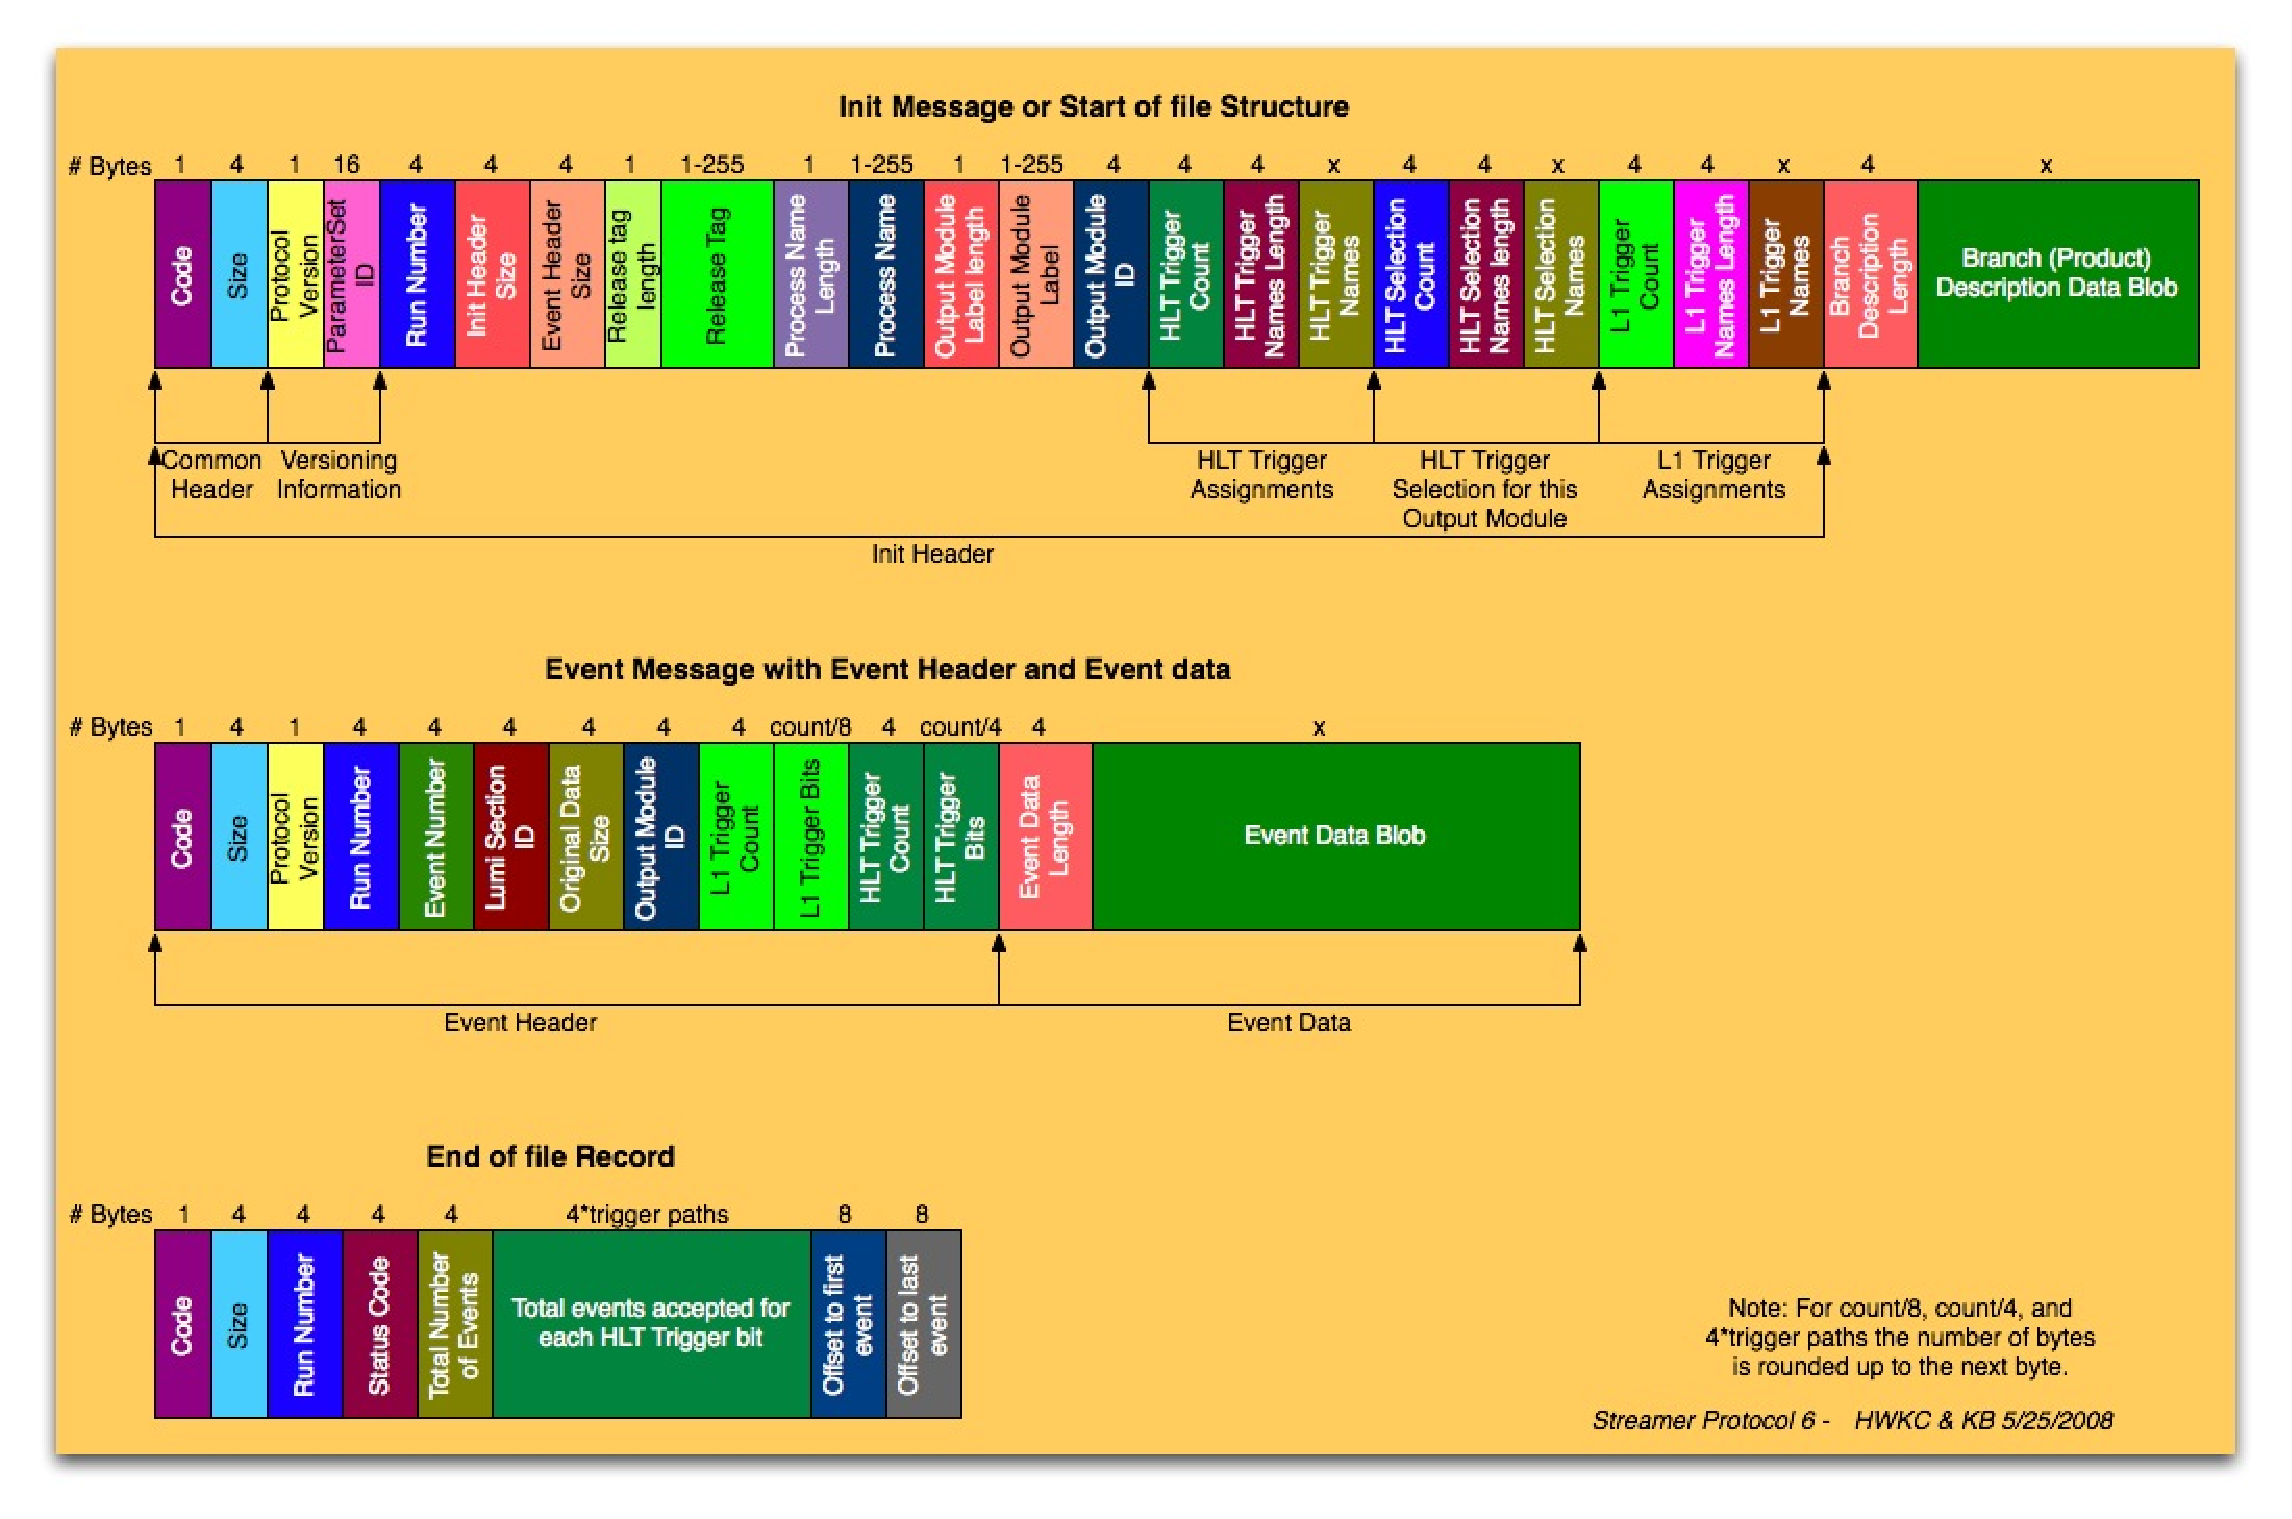
\includegraphics[width=6.0in]{Software/sm_mess_structure}
    \caption{Schematic showing the format of serialized data messages.}
    \label{fig:sm_mess_structure}
  \end{center}
\end{figure}

At the start of a run, each HLT process output module
sends an INIT message to the Storage Manager.
This INIT message is the same as the start of file record. For each run, the data 
for the first received INIT message of each output module
are saved for output as the start of file 
record for the streamer files. The data for each event is transmitted by the
HLT processes to the Storage Manager in the form of an event message which is
the same as the event record. It consists of the event header and the event
data. The event data is just the serialized ``data blob'' mentioned above
preceded by its size in bytes.

Besides the streamer files, the Storage Manager also writes out one index file
per streamer file. The format of these index files are given in Fig.~\ref{fig:sm_messages1}.
The index file contains the same start of file and end of file records as the streamer
file, however for each event it contains only the event header and the byte offset
for that event's data in the corresponding streamer file. The index file is intended
for use during Tier-0 processing to aid in random access reads of streamer files, and
is thus only temporary. The index file has the same name as the streamer file but with
an extension of ``.ind'' instead of ``.dat''. At this time, the Tier-0 group have yet to decide
if these index files will be used.

\begin{figure}[hbtp]
  \begin{center}
    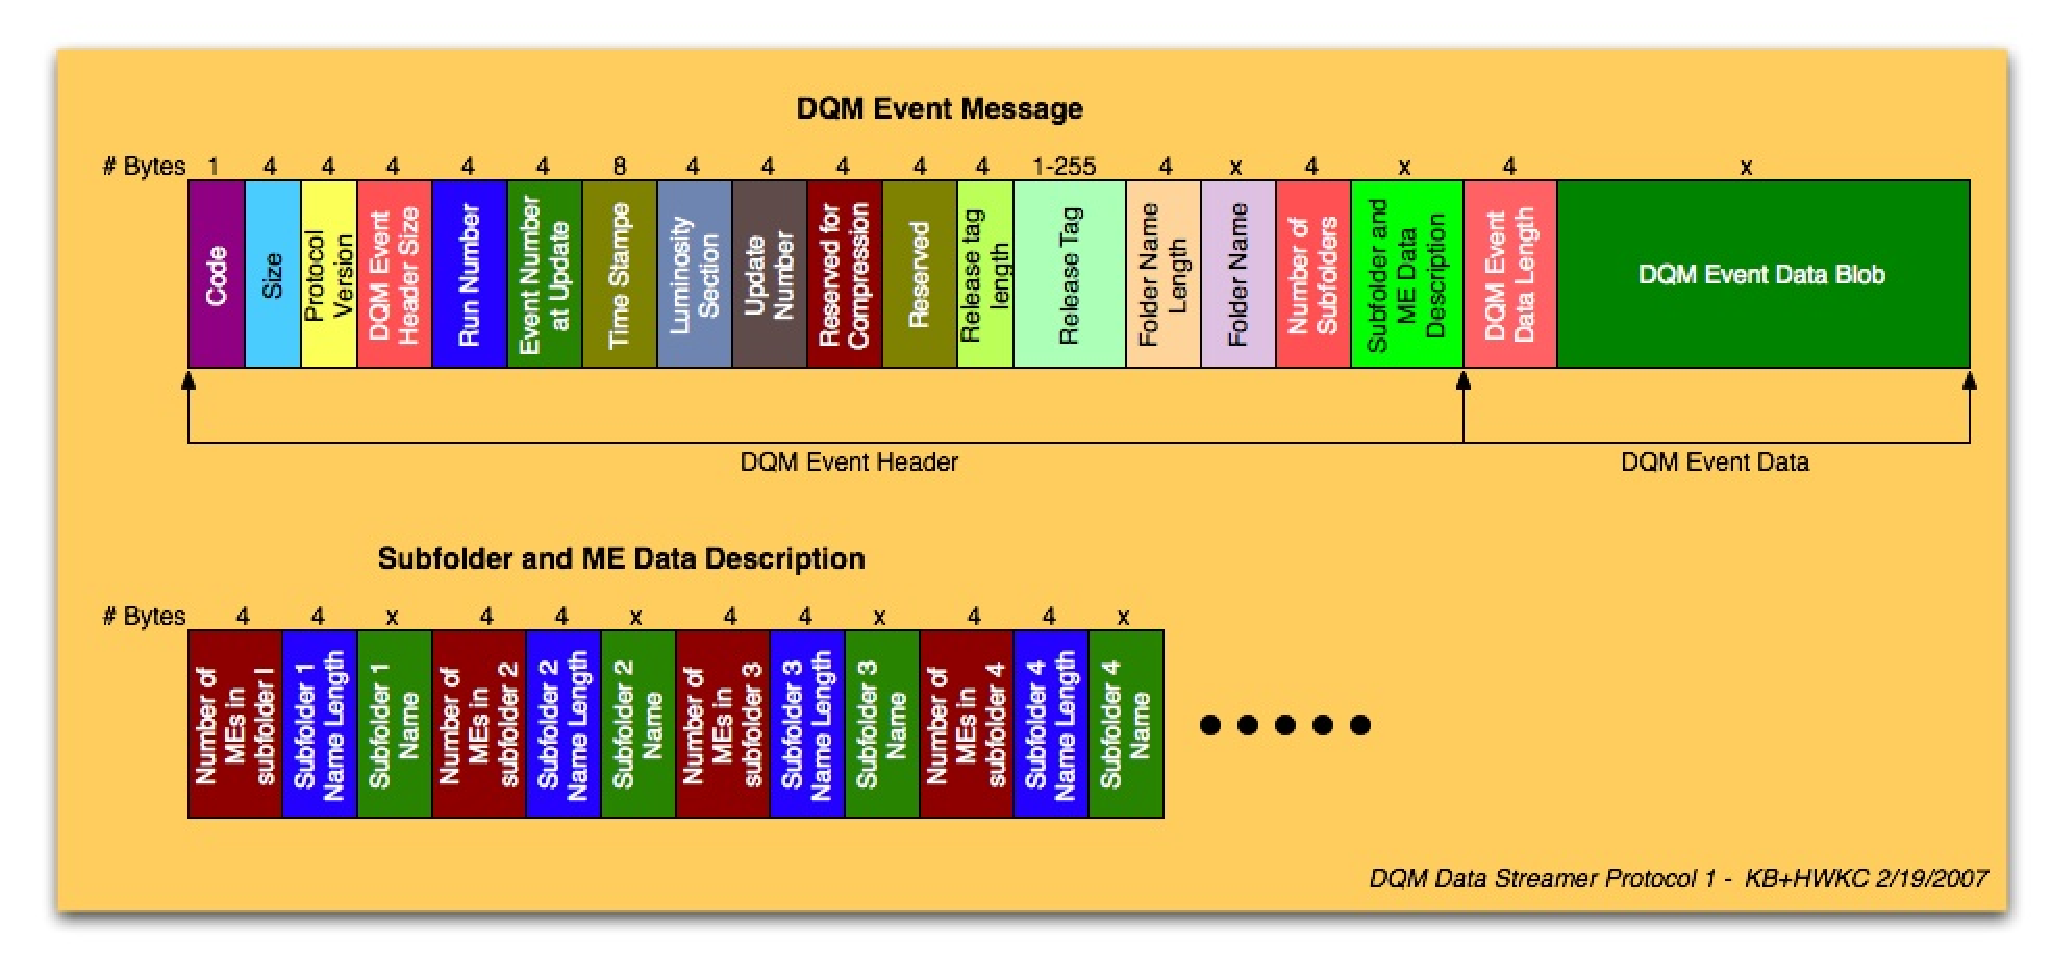
\includegraphics[width=6.0in]{Software/sm_dqmmess_structure}
    \caption{Schematic showing the format of serialized DQM messages.}
    \label{fig:sm_dqmmess_structure}
  \end{center}
\end{figure}

The transmission of DQM data from the HLT processes to the Storage Manager is done
using serialized DQM data messages. The format of these messages are given in
Fig.~\ref{fig:sm_dqmmess_structure}. The DQM data are essentially ROOT
histograms, and integers, floats, and std::strings stored as TObjects. These
data are organized into a number of (top-level) folders and subfolders. 

The DQM data for each top-level folder is serialized into a ``blob'' of bytes and
placed in its own DQM data message, and preceded by some header information as
shown in Fig.~\ref{fig:sm_dqmmess_structure}. The DQM data is sent at each
``update interval''. Usually this update interval is at the end of a luminosity
section (nominally 93~seconds).

Both the serialization of event data and the DQM data is done using ROOT.
The event data in the CMS framework is stored using ROOT TTrees, and
the serialization is done using the class descriptions of the event data
objects in ROOT for the particular version of the offline CMSSW version used. 
Only a subset of the event meta data is written out to the streamer file. 
%Normally it is assumed that the streamer file is the first step in the data chain, where
%the first process is the HLT process. Note that the HLT+SM is identified as
%a single process. This assumption has implications in the playback of real
% or MC data files in the online for testing purposes.
The chosen meta data are put into a data structure for which ROOT can generate
an automatic class description.

The start of file record in each streamer file includes the version of CMSSW used
and the ``branch descriptions''. These branch descriptions
 include the identifier of each of the event
data branches. However the class descriptions themselves are not stored in
the start of file record. To deserialize the data back to the original data objects
we load the class descriptions for each of the data branches using the 
appropriate CMSSW libraries. To be safe this means that the version of CMSSW
used to deserialize the streamer file should be the same as that used for
writing that streamer file. 

There is no provision for schema evolution for the
streamer files since they are temporary data formats. However this has implications
for the online event data consumers.

The DQM data contain
only histograms and simple types and std::strings, no special class descriptions
are needed to deserialize these data.


\subsubsection{Storage Manager Application}

The functions of the Storage Manager XDAQ application is listed below.

\begin{itemize}
\item Receive event data and DQM data in the form of I2O frames and
reform the fragments.
\item Output event data streamer files based on the per run configuration 
and the per event trigger bits.
\item Communicate with Tier-0 for the transfer of streamer files to Tier-0.
\item Take online consumer registrations and serve event data and DQM
data to registered online consumers.
\end{itemize}

After the experience with the first prototype of the Storage Manager it was
decided that no (real) processing is done in the Storage Manager application
since even the deserialization was found to be too CPU intensive for the
Storage Manager to keep up with the design incoming data rate.

\begin{figure}[hbtp]
  \begin{center}
    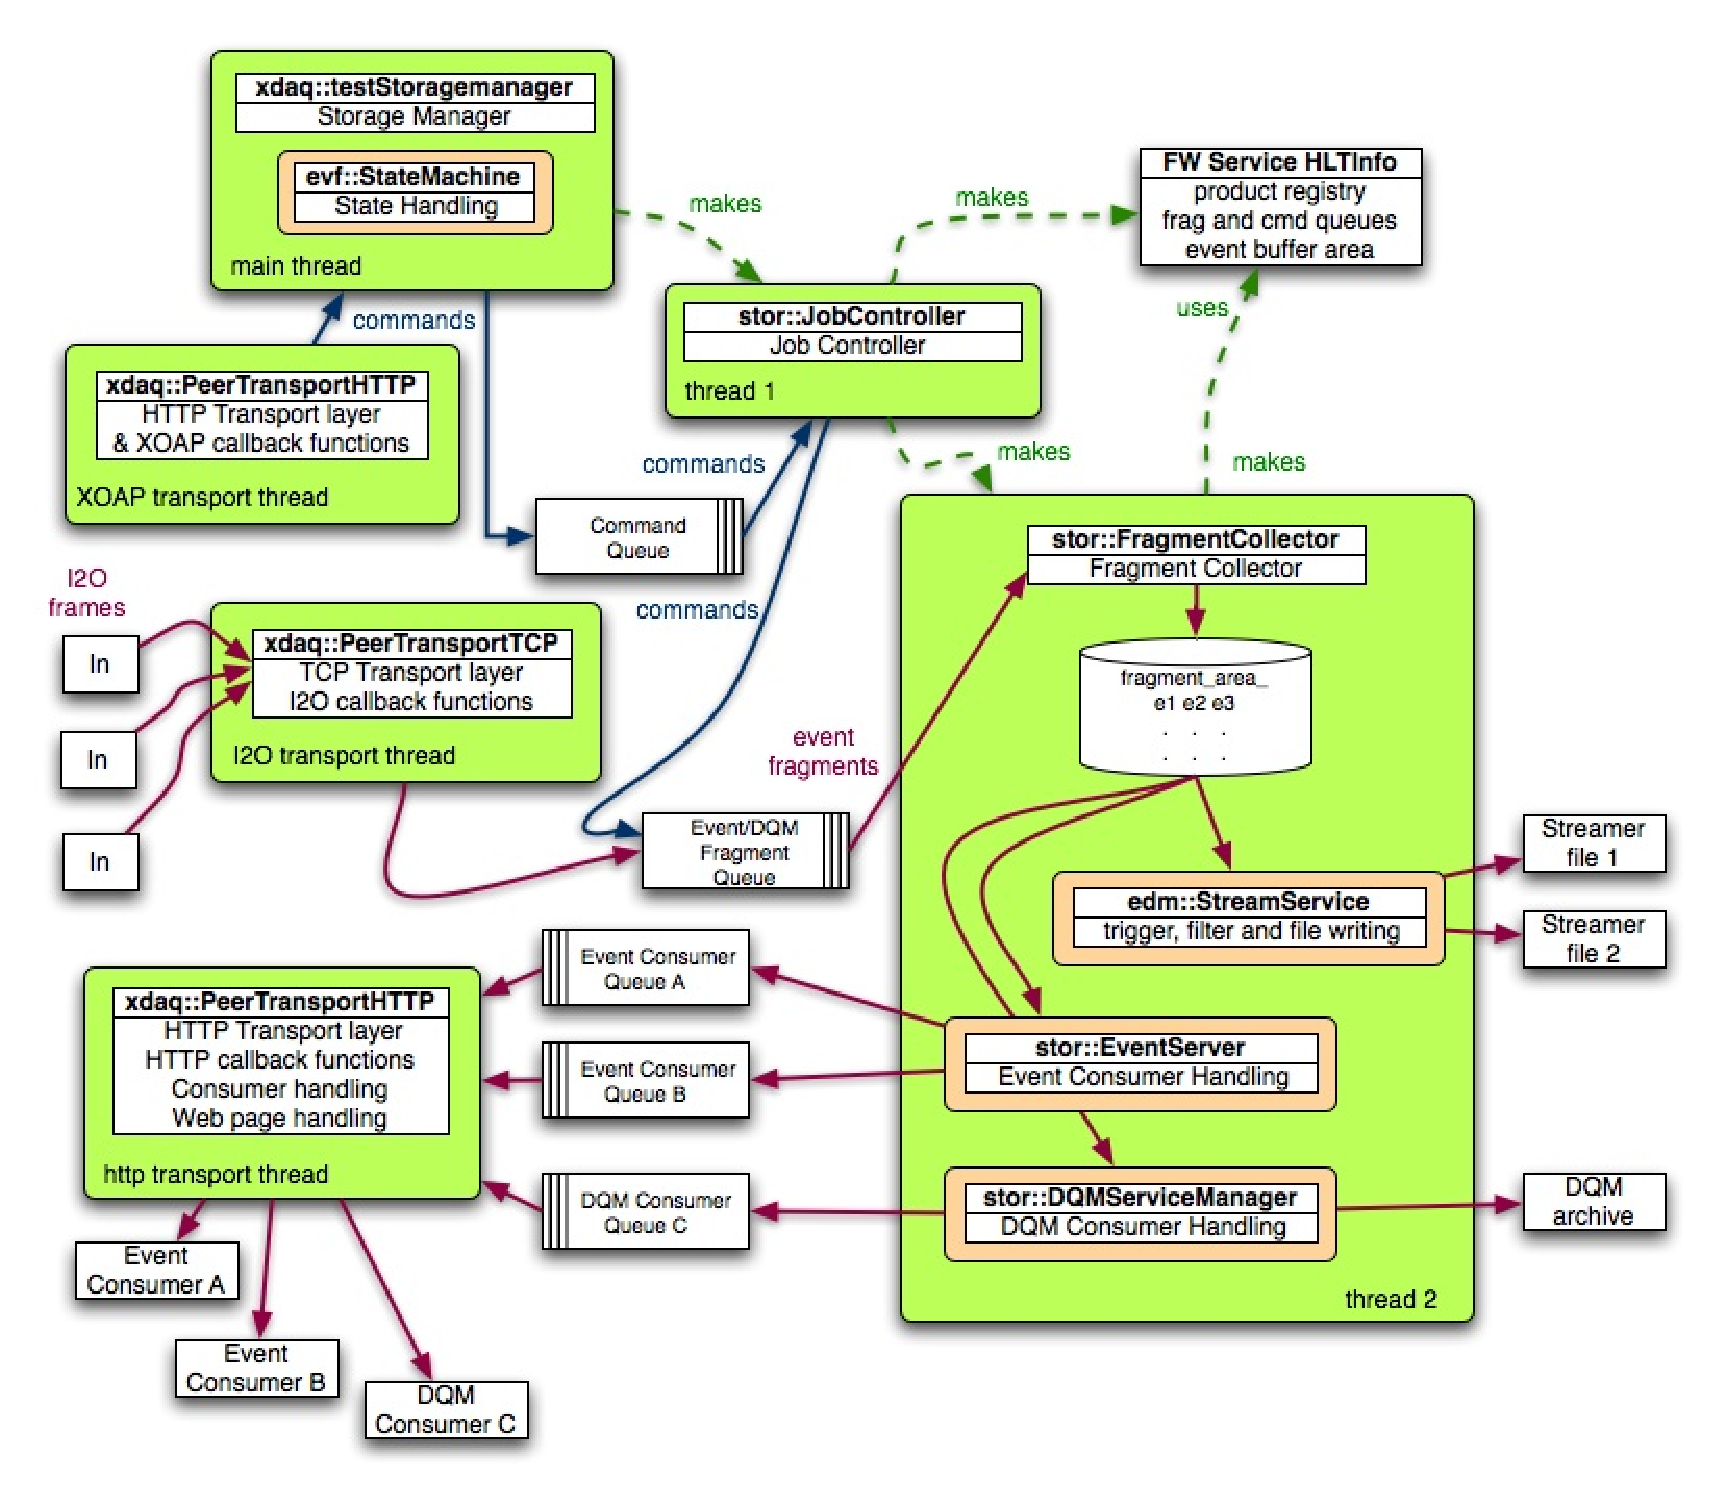
\includegraphics[width=6.0in]{Software/SM_System}
    \caption{Design of the Storage Manager application.}
    \label{fig:SM_System}
  \end{center}
\end{figure}

Figure \ref{fig:SM_System} illustrates the design of the Storage Manager
application. The StorageManager XDAQ application runs within the xdaq.exe
executable in the main thread,
but basically all the processing is done in other threads of this application.
There are three transport callback threads, one for I2O, one for XOAP, and one
for HTTP.  Additionally there are two other threads started originating from the
StorageManager application itself, the JobController thread, and the
FragmentCollector thread. The functions of these processing threads are
given below.

\begin{itemize}
\item {\em XOAP transport thread.} Commands to the Storage Manager are sent
via XOAP (XML) messages, and various XOAP callback functions are defined in
the Storage Manager application to handle these commands. These commands
include commands to configure, start, pause, and end (halt)  the
Storage Manager application.

\item {\em I2O transport thread.} The incoming event data and DQM data I2O frames
trigger I2O callback functions that run in the I2O transport thread. The I2O callback
functions are defined in the Storage Manager application and essentially just place 
the appropriate data fragments with identifiers into
the event/DQM fragment queue. If the SM instance is run on a PC with multiple
network interface cards (NICs), there can be one I2O transport thread per NIC.
The event/DQM fragment queue is protected by a mutex.

\item {\em HTTP transport thread.} HTTP callback functions are also defined in
the Storage Manager application and handle various tasks. The tasks include
generating web pages with various monitoring data about the Storage Manager,
called application web pages and these are the most direct means of monitoring
each XDAQ application besides looking at that application text console. Other
HTTP callback functions handle online consumer registration and sending data
to the online consumers.

\item{\em JobController thread.} The JobController creates shared data structures like
the fragment queue and creates and starts the FragmentCollector thread. The Storage
Manager can issue commands to the JobController thread by placing them in the
command queue. In the running state the JobController thread just reads the
command queue and reacts to what is read. The command queue is a blocking queue
so that if empty a read will block until something is placed in the command queue. The 
command queue is protected by a mutex.

The JobController thread can control the FragmentCollector thread by placing
commands in the (event/DQM) fragment queue. The fragment queue is a blocking
queue like the command queue and also protected by a mutex.

\item{\em FragmentCollector thread.}  In running mode the FragmentCollector thread
reads the fragment queue and processes event fragments, DQM data fragments,
and also commands like an end of run or a halt. The data fragments are collected and
reformed into the serialized event data or DQM data. 

Once reformed the serialized data for an event is written out to streamer files based
on the trigger bits for the event and the initial per run configuration of the Storage Manager.
The output files can be written out in streams, for example a physics stream, a
calibration/alignment stream, and a debug stream. In each SM instance,
the data for each luminosity section
for each stream is written to one file. The data for the event is also passed to the
event server which determines if it needs to be placed in any online consumer queues.

Reformed DQM data is passed to the DQMServiceManager which can be configured to sum up
histograms for the same update. Once the histograms are summed they are written out to
the DQM disks. These DQM data are also passed to the
DQMEventServer which determines if it needs to be placed in any DQM consumer queues.
\end{itemize}

The state of the StorageManager application is kept in a Finite State Machine. This
is implemented using FSM code provided and maintained by the Event Filter Group
which is part of the CMS DAQ group. This provides a uniform set of states and
allowed transitions for XDAQ applications within the Event Filter Group. The
state chart for the StorageManager application is illustrated in Fig.~\ref{fig:sm_fsm_chart}.

\begin{figure}[hbtp]
  \begin{center}
    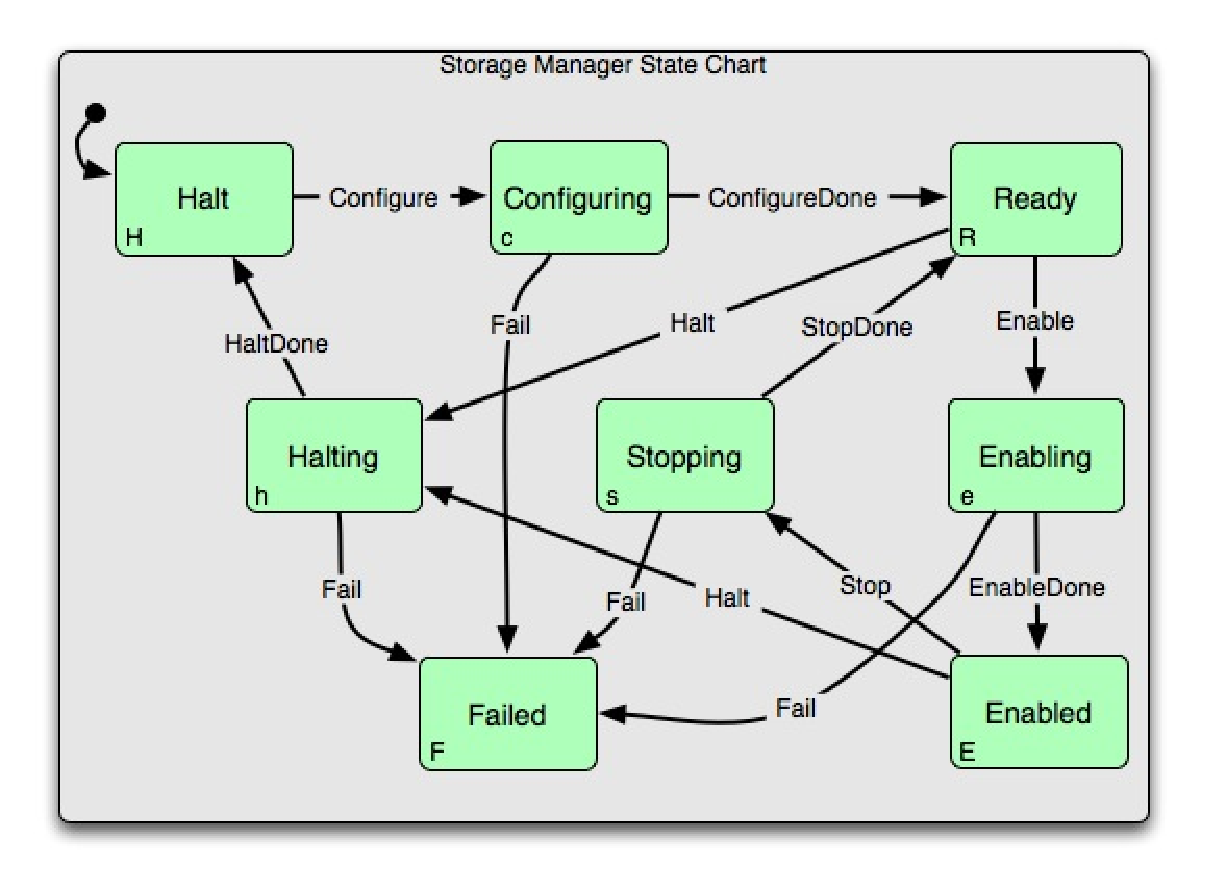
\includegraphics[width=4.5in]{Software/sm_fsm_chart}
    \caption{Storage Manager State Chart}
    \label{fig:sm_fsm_chart}
  \end{center}
\end{figure}

The online event and DQM consumers interact with the Storage Manager event and
DQM servers through HTTP GET and POST commands, and data are transferred using
a binary stream. Online consumers register with the Storage Manager and get
data via a pull mechanism, polling at a maximum rate of a several Hz. The
event and DQM servers limit the data rate and bandwidth to online consumers to
ensure that the primary function of the Storage Manager is not compromised.

Copies of the data are minimized in the Storage Manager during its execution
loop. The received data fragments remain in the XDAQ memory pool
until all fragments are received. At this point the data is copied and
concatenated together to reform the serialized ``data blob" before being
written out to streamer files. The memory for this event data in the
XDAQ memory pool is
then released, but the event server retains a
copy of this event data. Pointers to this single copy of the data
are used in the consumer queues.


\subsubsection{Storage Manager Proxy Server Application}

With multiple StorageManager instances, one for each subfarm, online
consumers must be able to get events from multiple Storage Managers. This is
one of the functions of the SMProxyServer XDAQ application. The design of the
SMProxyServer is illustrated in Fig.~\ref{fig:SMProxyServer_System}.

\begin{figure}[hbtp]
  \begin{center}
    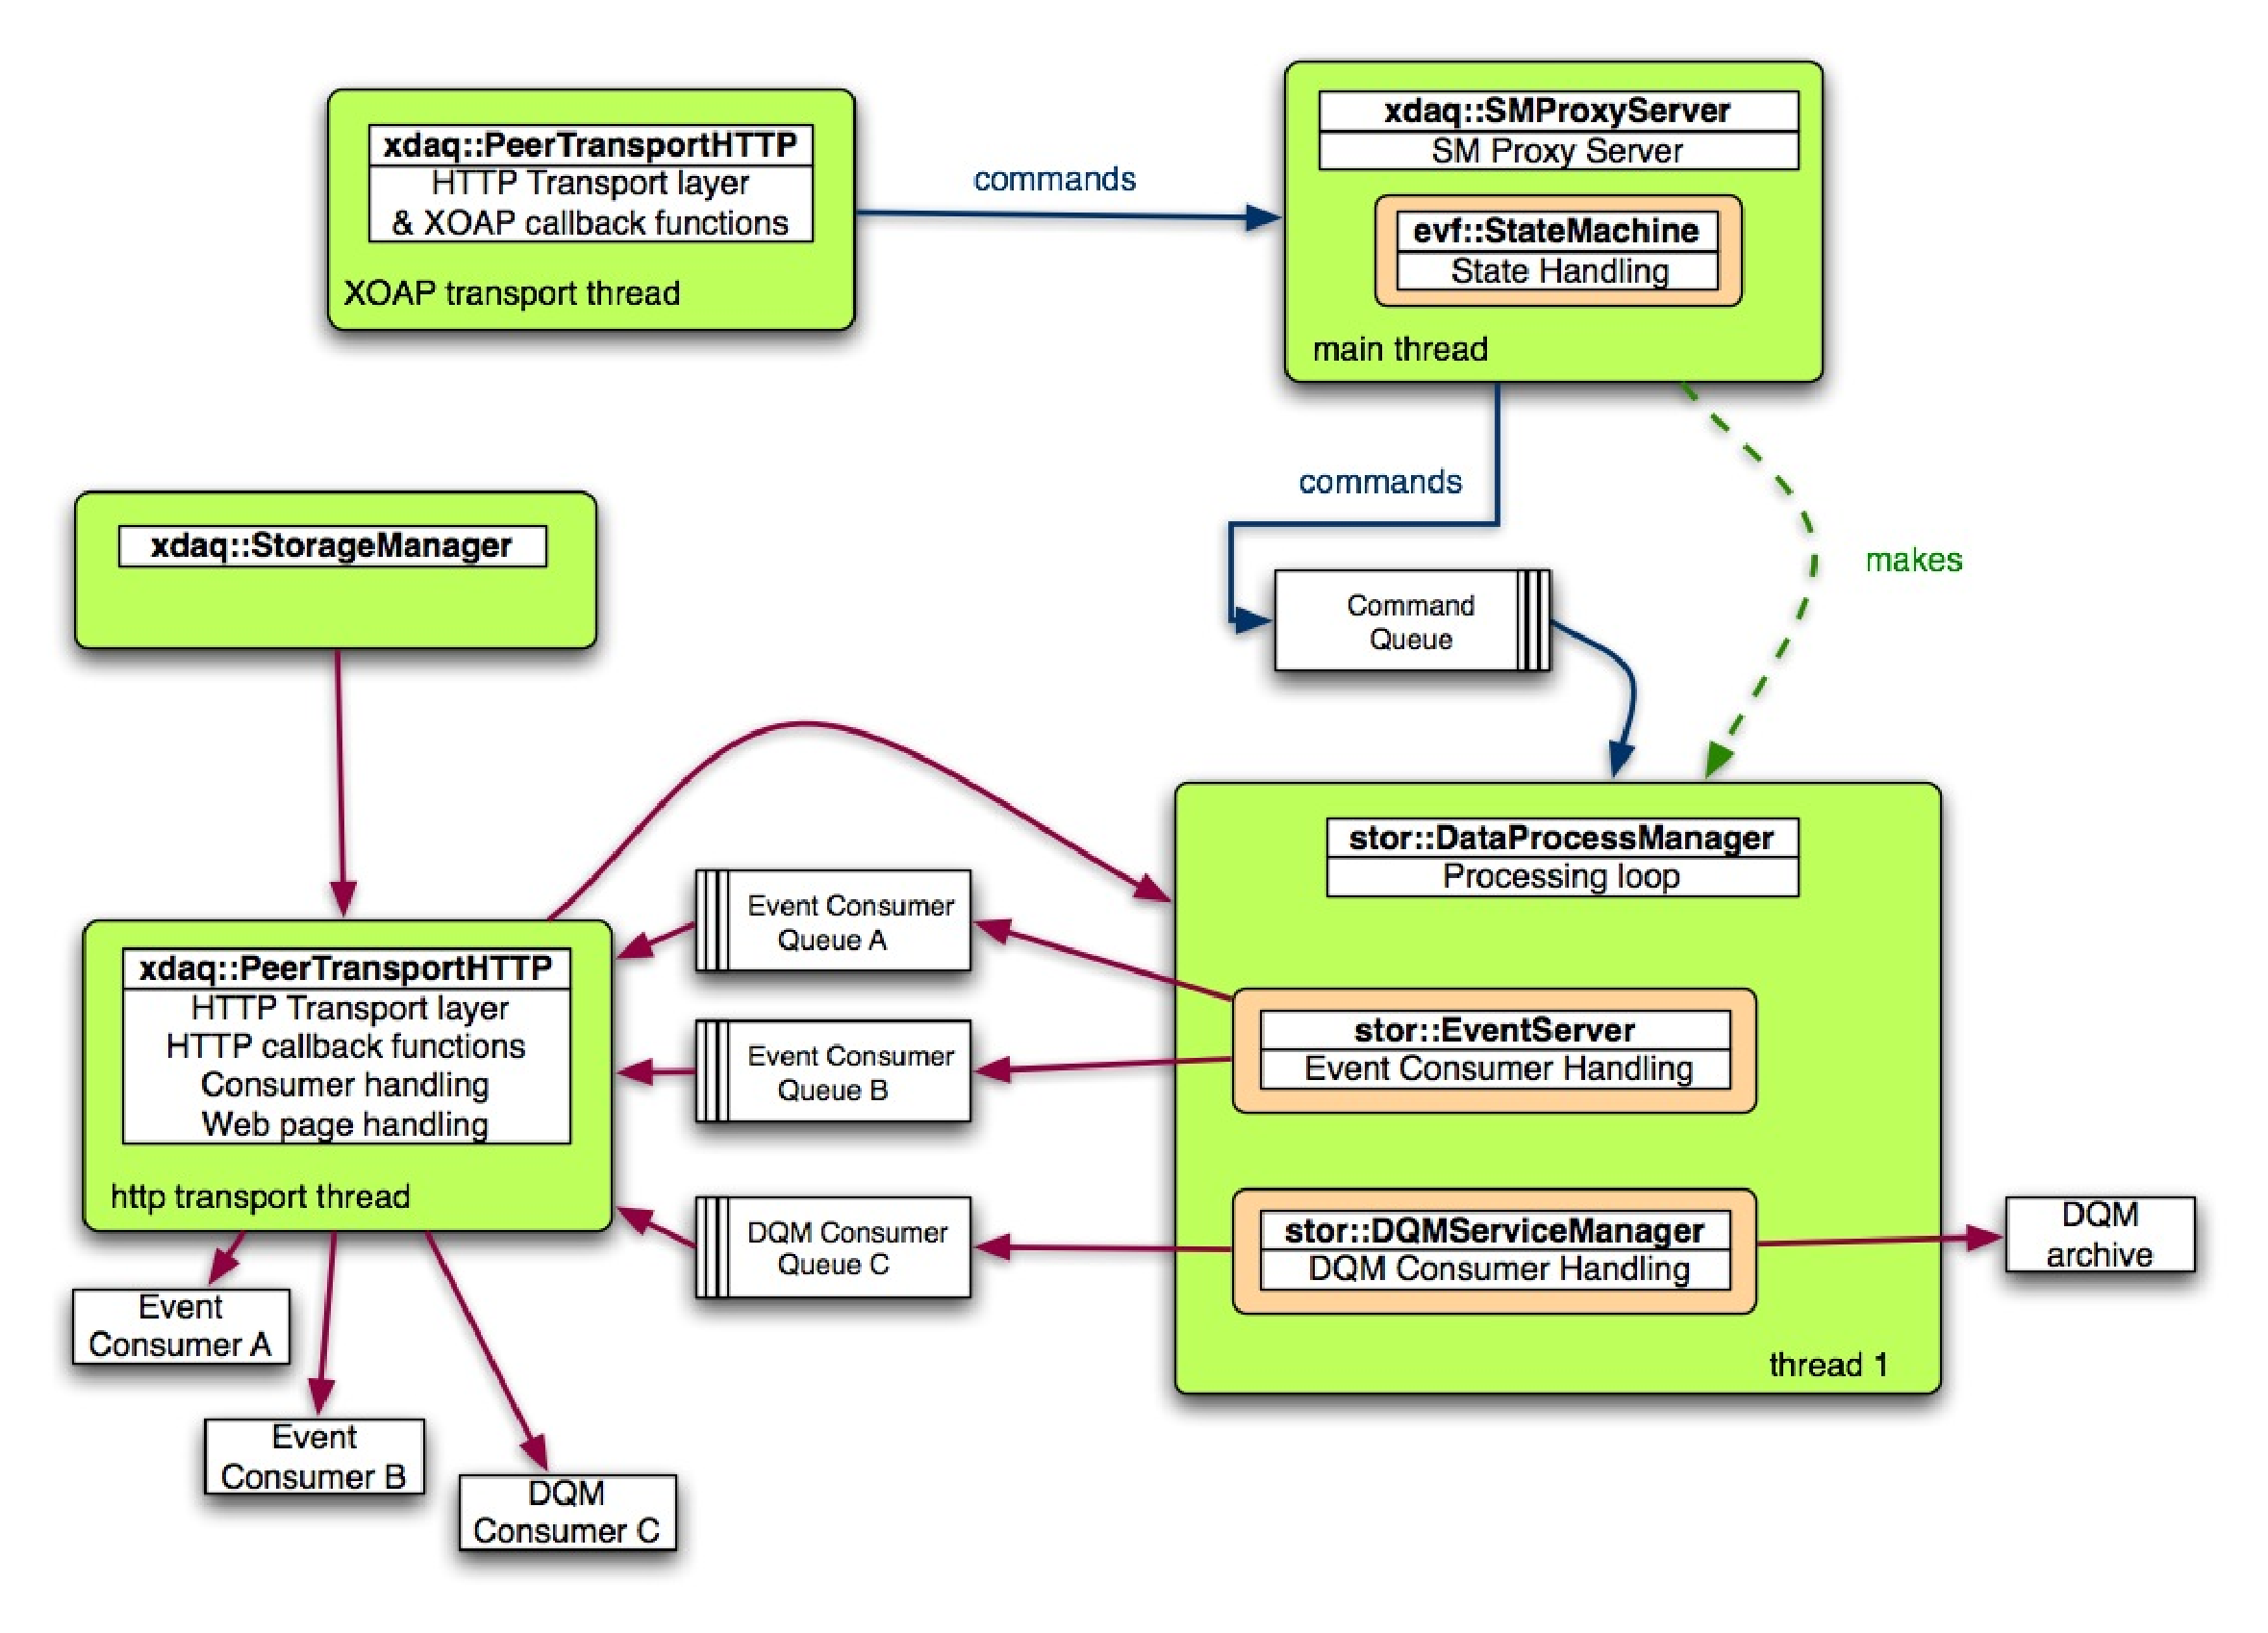
\includegraphics[width=5.5in]{Software/SMProxyServer_System}
    \caption{Design of the Storage Manager Proxy Server application.}
    \label{fig:SMProxyServer_System}
  \end{center}
\end{figure}

The SMProxyServer gets event data and DQM data from each of the StorageManagers
like an online consumer. The SMProxyServer also
registers itself with each of the StorageManager applications. However unlike
a regular online consumer, the SMProxyServer can receive data from
multiple HLT output modules.  The event server in each SM instance can
limit the rate of the data to the SM Proxy Server.

As much of the StorageManager code as possible is used in the
SMProxyServer to reduce the amount of code that needs to be maintained.
Instead of the JobController thread and the FragmentCollector thread the
SMProxyServer only has a DataProcessManager thread. This DataProcessManager
thread manages the registration of the SMProxyServer with all StorageManager
instances, and processes commands in the command queue.

The SMProxyServer functions as an event and DQM server to serve online consumers.
In normal running the online consumers would actually only connect to the
SMProxyServer application. This isolates the StorageManager applications from
the online consumers.

Finally the SMProxyServer receives DQM data from each of the StorageManager
applications and sums up the histograms from each StorageManager instance
for the same update and saves them to the DQM disk.

The SMProxyServer application uses the same state machine code as the 
StorageManager application and the state chart is the same as that given
in Fig.~\ref{fig:sm_fsm_chart}.


\subsection{\label{sec:fpt0}File Processing, and Communication and interaction with Tier-0}

For each stream and each StorageManager instance one output file is written
per luminosity section. Each SM instance uses volumes on separate disk arrays 
(see the hardware section, Section~\ref{sec:stohard}).

Events arrive asynchronously to the Storage Manager depending on the processing
time for each event in the HLT process. On the arrival of an event from a
new luminosity section a new streamer file is created for this luminosity section,
and an entry is created in the online database for this file. 
The arrival of an event from the next
luminosity section to a StorageManager will start a timeout counter. Once this
timeout is reached all files for the previous luminosity section is closed.
The database entry for each of the closed files are updated. The information
updated includes the number of events in the file and a file CRC checksum.
The files are moved to a staging subdirectory and the Tier-0 system is notified
using a shell script provided by the Tier-0 group.

The database creation, update and the Tier-0 notification is done asynchronously 
outside of the SM application. The SM application writes a logfile that is monitored 
by a daemon (called ``InjectWorker'' written in PERL) running on the same node. 
On arrival of new information
in the log file the daemon handles the necessary database interactions. It verifies
if the information entered on opening of the file is consistent with the information on 
closing of the file, and updates the necessary fields known only when the file is closed
(e.g.~the CRC checksum and the file size). On successful verification the information is
passed to the Tier-0 notification script. The files get independently transferred by 
a daemon of the transfer system (called ``CopyWorker'' written in PERL).
The file size and checksum recorded in the database of each so copied file with be verified 
on the T0 side. For every successfully copied file the T0 system will update a field in the 
database indicating that the file was successfully transferred.
A separate PERL script~(launched by a cron job) monitors the status of each of the 
closed streamer files via the database and manages the removal of streamer files.

In addition to the code, all scripts used in the Storage Manager are maintained by 
the Storage Manager group reside in CVS along with all the C++ code.


\subsection{Control, Monitoring, and Error Handling}

\subsubsection{Control}

The behavior o the Storage Manager application
is controlled by configuration data that are read by the Storage Manager 
during the transition from Halt state to the Ready state. A new run is always
started when the Storage Manager is configured or reconfigured. The configuration
data determines what streams the Storage Manager will write out, and the selection of
trigger and HLT output module id for each stream. The configuration data also specify which
disks will be written to, and govern the setup of the event server and DQM
server, as well as various other parameters that govern the monitoring behavior within the 
StorageManager and SMProxyServer applications.

Control of the Storage Manager is done by the CMS Run Control using XOAP messages.
These XOAP messages triggers the state transitions. If problems occurs during the
state transition the Storage Manager will go into the Failed state instead as
illustrated in the state chart, see Fig.~\ref{fig:sm_fsm_chart}. 

The XOAP messages are sequenced and sent by a set of Java applications called
Function Managers (FM). These Function Managers react to events (XOAP messages) from
both the Function Managers that control them, and to events from the XDAQ applications
that they control. The SM instances are under the DAQ FM while the SM Proxy Server
application is controlled by the DQM FM. In a later update the SM Proxy Server application
will move to being controlled by the DQM FM. The DQM FM is created and maintained by
the CMS central DAQ group while DQM FM is created and maintained by the
CMS DQM group. 
The hierarchy of Function Managers are illustrated in Fig.~\ref{fig:fm_example}.

\begin{figure}[hbtp]
  \begin{center}
    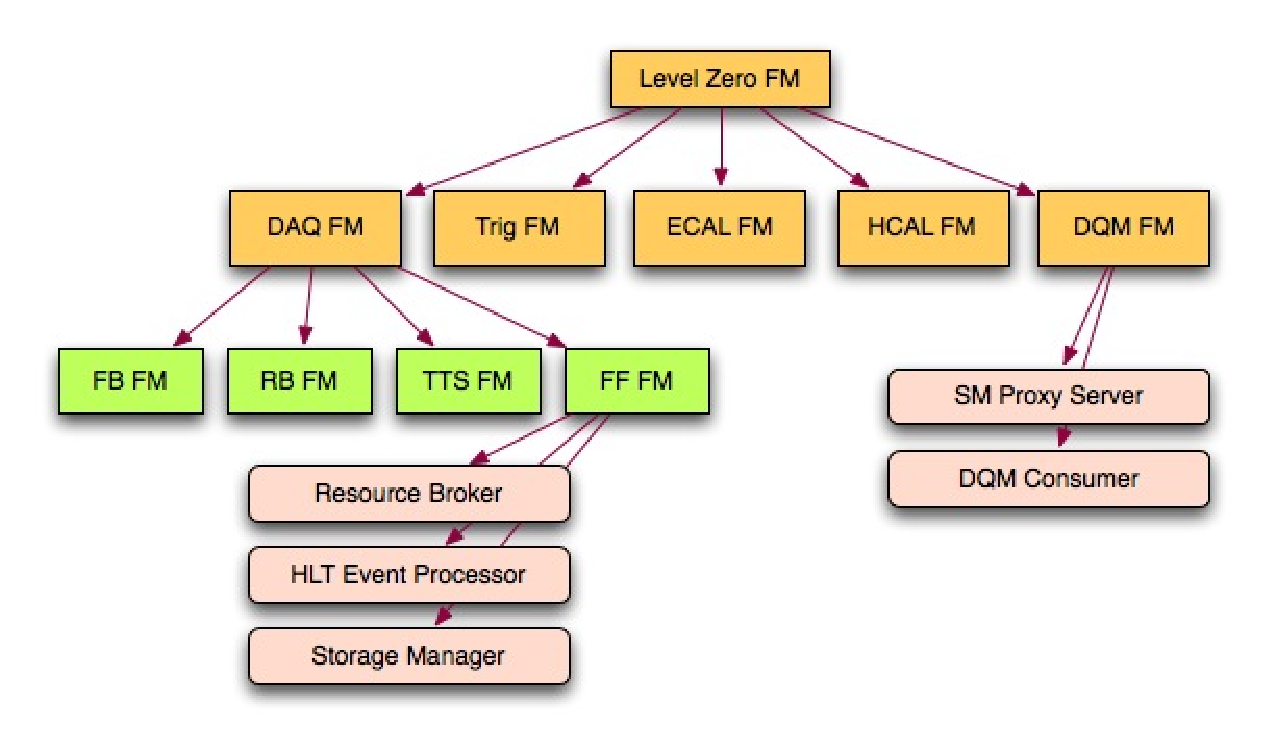
\includegraphics[width=4.5in]{Software/fm_example}
    \caption{Illustration of the hierarchy of Function Managers.}
    \label{fig:fm_example}
  \end{center}
\end{figure}

\subsubsection{Monitoring}

There are different levels of monitoring implemented for the Storage Manager
system, from the lowest level closest to the StorageManager and
SMProxyServer XDAQ applications, to higher levels where the monitoring
data has to pass through additional software.

Monitoring of the software at the lowest level is via the XDAQ application
console and the XDAQ application web pages. The console just contains text
that is output from the application. Different levels of text are generated
depending on their information content or severity, {\em i.e.} debug, 
informational, warning, and error levels. The text that appears from an
application can be filtered and also directed to specific consoles. These
text messages are created using the standard offline framework message logger
integrated with the online messaging system.

Each XDAQ application contains
a simple HTTP server that can serve web pages to a browser. The StorageManager
and SMProxyServer applications both have a number of monitoring web pages defined. 
These monitoring pages are dynamically generated when a browser requests
a specific web page. The monitoring pages include information on each HLT node
sending data like the node address, data rate, and latency. For the Storage
Manager itself, some information that is currently included are the status of the
XDAQ memory pool, the total maximum, minimum, and average data rate into and
out of the StorageManager, the average event size, the number of events received,
and statistics for the each streamer file written or being written. Other web pages
give the status of connected consumers and the status of the event and DQM servers.

Although a lot of information on the software status is available at the lowest 
level if needed, typically we minimized the processing the Storage Manager has 
to do to processes incoming web page requests. We make use of other monitoring
features of XDAQ. A list of important properties
of the Storage Manager is defined at configuration time and the Storage Manager
updates the information for this list. The list is accessible by other online
applications like the CMS Run Control. The values of the list of quantities are
published in the online XDAQ monitoring system and saved to a database from
which any number of applications
can access this information.

Standard web pages are generated using the monitoring lists for each XDAQ
application. Each online subsystem has a single web page summarizing the
status of that subsystem, called its ``Page One''. The Storage Manager Page One
has information mainly about the status of streamer files, and the status of
the output disk system. An example of the Storage Manager Page One is given
in Fig.~\ref{fig:sm_page1}.

\begin{figure}[hbtp]
  \begin{center}
    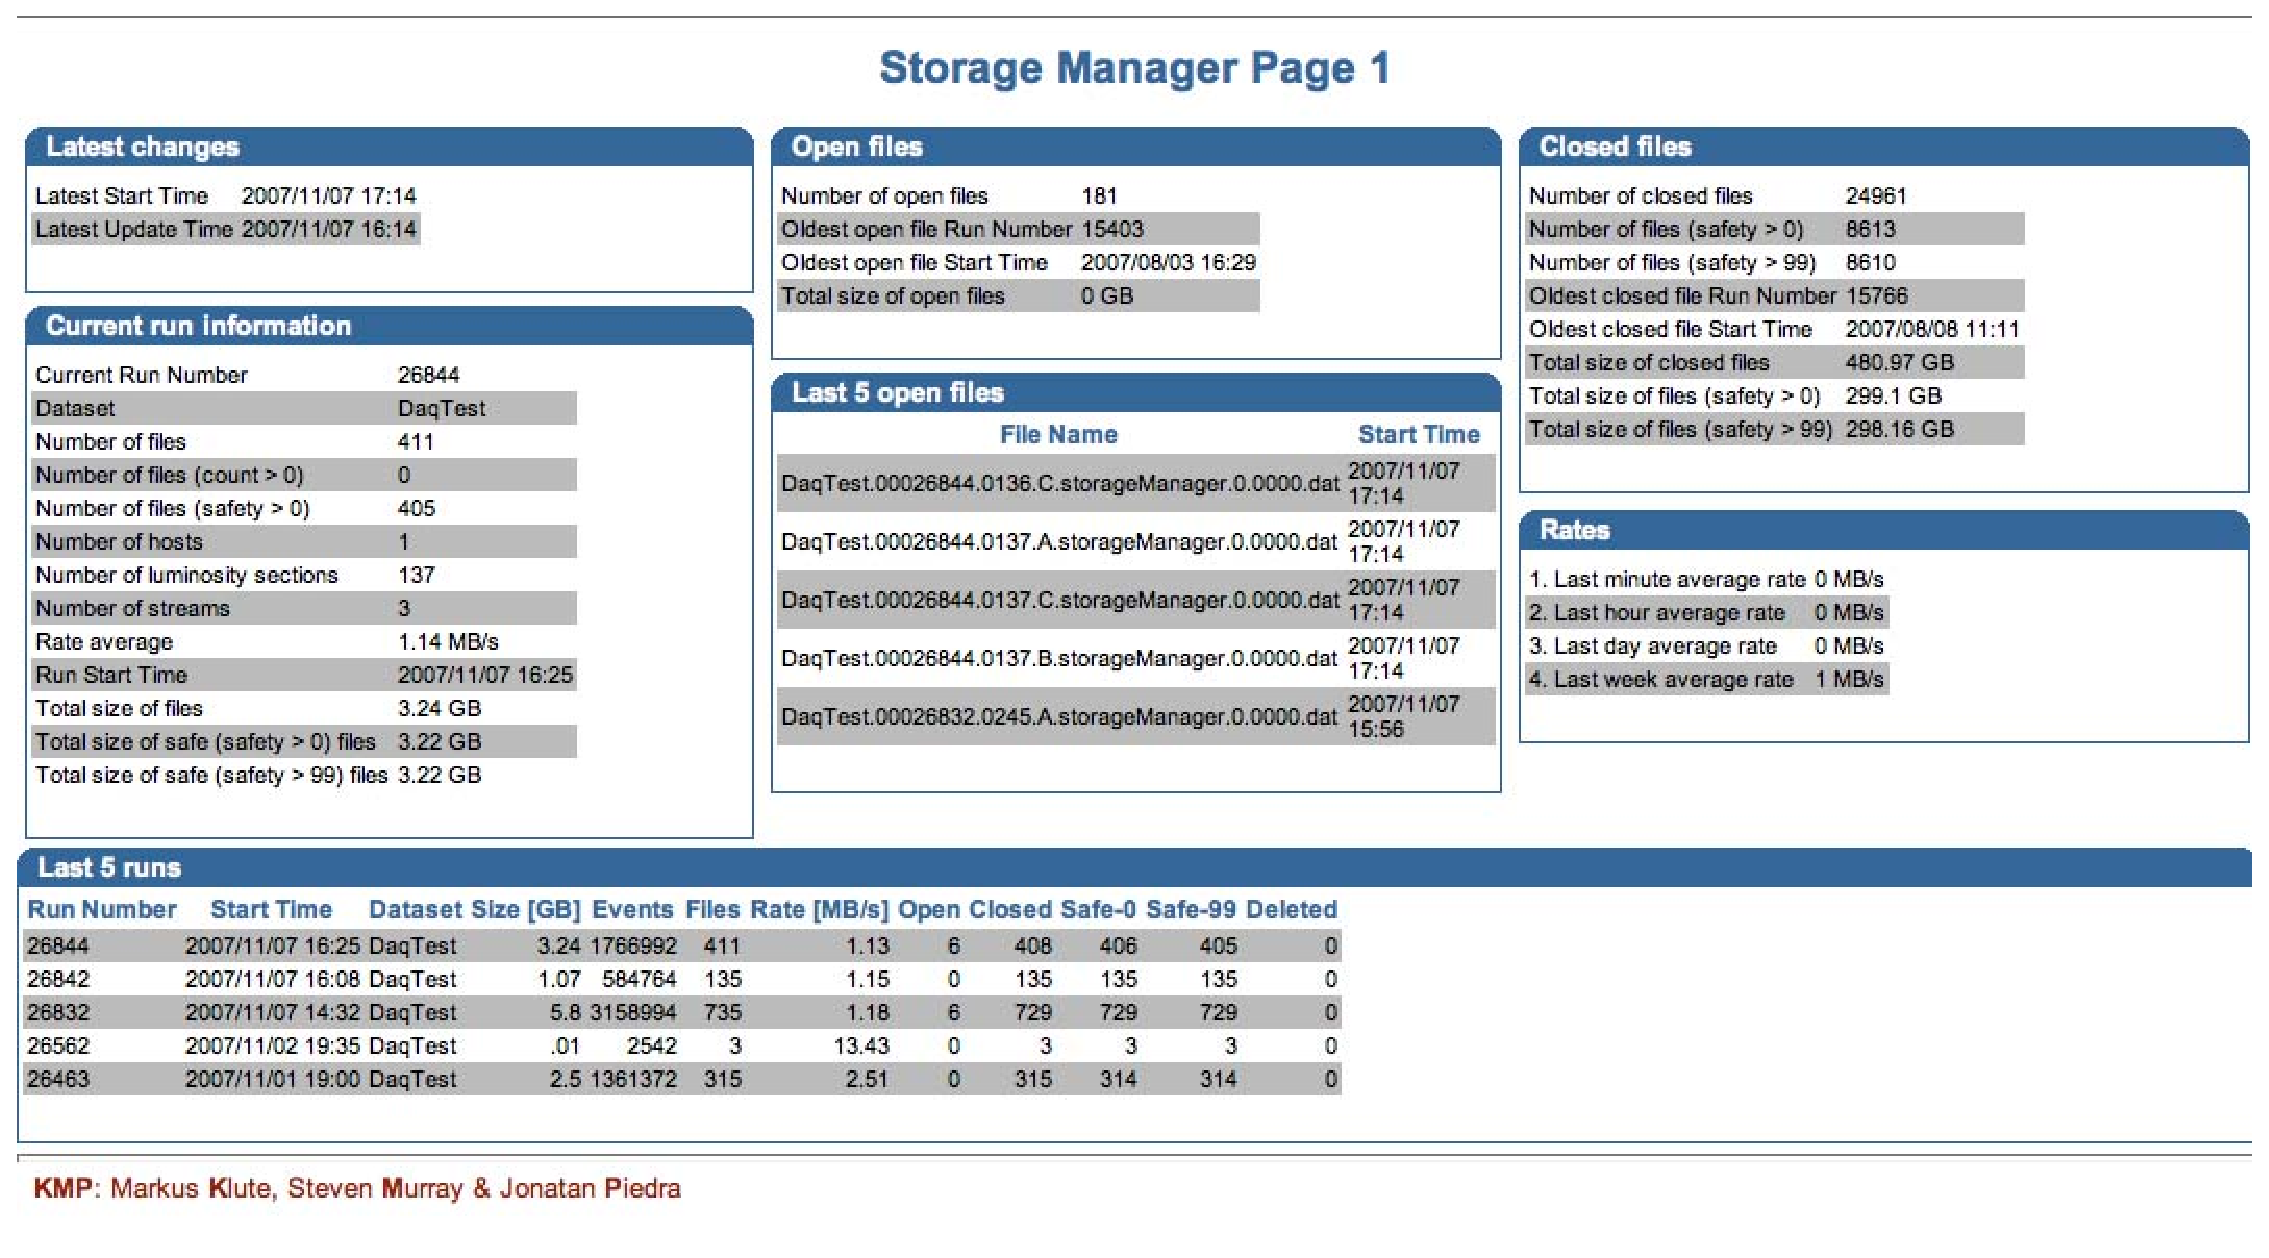
\includegraphics[width=5.5in]{Software/smpage1_example}
    \caption{Image of the Storage Manager Page 1 monitoring web page.}
    \label{fig:sm_page1}
  \end{center}
\end{figure}

The error alert system in the CMS online is still under development, and part of
the work of the SM group will be to integrate into this system when ready. In
addition the SM group is working on providing more monitoring and check-pointing
to help analyze problems that may arise, and to provide more useful information
for non-SM experts.

The monitoring of the Storage Manager hardware will be covered in the
hardware section.

\subsubsection{Error Handling}

There is currently some limited error handling in place for the Storage Manager,
mainly to handle the various error conditions so far experienced in the CMS global
cosmic ray data taking exercises. Handling of foreseen error conditions forms 
the major part of active code development for the Storage Manager group.
Currently most of the errors that are handled are considered fatal ones, and these
will cause the Storage Manager to go to the Failed state with an associated error condition 
message. Besides considering foreseen error conditions we have also received
experience from actual running of the system,
situations causing problems are analyzed and code changes for more monitoring
or error handling implemented if appropriate.

There are unit tests in place for the data serialization and deserialization code,
and for the streamer message creation and access. These unit tests are run during
each CMSSW pre-release and the production release to ensure that these code
function properly. The tests of the StorageManager and SMProxyServer applications
relies on a number of applications and already constitutes an integration test.
These tests are currently initially done manually on a test system consisting of two nodes.

The next validation tests are done on a CMS development system at the experiment,
the cmsdaqpreseries (Green Barrack) cluster. This system has installed the normal
CMS online with full Run Control and other features that enable tests of the SM system
software in a realistic online environment. The software development team has access
to this system and is being trained on operating it from Fermilab.
It is possible that many problems seen during 
data-taking can be reproduced in the cmdaqpreseries system and analyzed.
Currently scale tests and tests involving the actual SM hardware (disk arrays) are not
possible in the cmdaqpreseries cluster.
Scale and performance tests are done by the SM operations team on the actual SM hardware,
and a part of the CMS online system.

CMS has had a number of DAQ global run exercises and the Storage Manager is
an integral part of every global run exercise. The Storage Manager system is
scale tested up to the maximum foreseen rates
during these global exercises. Any problems or issues in each run
are diagnosed and corrected before the next global run exercise. Additional
functionalities or features of the Storage Manager may also be tested in the
global run exercises and in test running between these exercises.

Currently we are still collecting data on the types of error conditions we
face from the global run exercises, however we have created a  fault tolerant and 
error recovery policy. This policy is still awaiting feedback from the central DAQ group.
We will ensure that this error handling policy is an integrated policy that fits in with the CMS
online plan for fault tolerance and recovery.

Table \ref{tab:fc_errorhandling} gives the error handling policy proposed 
to the central DQM group.

\begin{table}
\begin{center}
\caption{\label{tab:fc_errorhandling}Error Handling Policy for Storage Manager 
Software Components.}
\vspace*{3mm}
    \renewcommand{\arraystretch}{1.5}
    \setlength{\tabcolsep}{2mm}
\begin{tabular}{| p{0.27\textwidth} | p{0.25\textwidth} | p{0.45\textwidth} |}
\hline
\multicolumn{3}{c}{\bf FragmentCollector} \\ \hline
{\bf Problem} & {\bf Cause} & {\bf Desired Reaction} \\ \hline
Corrupt data received from HLT such as invalid message types &
   Logic problems in upstream applications or memory corruption &
   Log error, keep statistics, discard fragment, (and all other fragments 
   for this event and output module). Keep running. \\ \hline
Unrecognized data (unexpected fragment type) & 
   Logic problems in upstream applications or memory corruption &
   Log error, keep statistics, discard fragment. \\ \hline
Missing fragments &
   Drop packets? &
   Provide timeout, log error, keep statistics, discard the partial event. \\ \hline
Out of order fragments & &
   Update the code to handle out of order fragments so that this is not a problem.
   Keep statistics � believe should not happen with tcp.\\ \hline
System exception &
   Exception thrown in a system call, or fatal error related to a system call, e.g. problem 
   writing to disk, no room on disk &
   Transition to a Failed state and log an error message. \\ \hline
Application exception &
   Exception thrown within the Storage Manager code. &
   For exceptions that are understood and can be handled, log them, keep statistics, and 
   discard fragment.  For exceptions which can not be handled, transitions to a Failed state 
   and log the error.\\ \hline
Incoming fragment causes application exception &
   Error decoding header, decoding DQM fragment with Root &
   Same as Unrecognized data (unexpected fragment type)\\ \hline
Event message view - bad protocol version & &
   Log error, keep statistics, discard fragment.\\ \hline
No event server &
   Logic error &
   Transition to a Failed state and log an error message? Or Just log error, 
   set monitoring alert and keep running?\\ \hline
Writer error & & See below\\ \hline
Wrong run number & Data from a mix of runs sent to the SM &
   [Update the code to determine the run number in a better way than from the cfg file.]  
   For events with the wrong run number, Log error, keep statistics, discard fragment.\\ \hline
Invalid fragment key &  & Log error, keep statistics, discard fragment.\\ \hline
Fragments in the queue after done message received & &
   Discard fragments, generate error message.\\ \hline
Could not stop writer properly & &
   Transition to a Failed state and log an error message.\\ \hline
Could not stop DQM event server properly & & 
   Transition to a Failed state and log an error message.\\ \hline
\end{tabular}
\end{center}
\end{table}

\begin{table}
\begin{center}
\vspace*{3mm}
    \renewcommand{\arraystretch}{1.5}
    \setlength{\tabcolsep}{2mm}
\begin{tabular}{| p{0.27\textwidth} | p{0.25\textwidth} | p{0.45\textwidth} |}
\hline
\multicolumn{3}{c}{\bf ServiceManager (writer)} \\ \hline
{\bf Problem} & {\bf Cause} & {\bf Desired Reaction} \\ \hline
Cannot write to a file & & Transition to a Failed state and log an error message.\\ \hline
Cannot create a file & & Transition to a Failed state and log an error message.\\ \hline
No space on disk & & Transition to a Failed state and log an error message. 
   Implement watermark alerts as disk partitions fill up.\\ \hline
Misconfiguration & & Transition to a Failed state and log an error message.\\ \hline
Event from closed lumi section (no test now) & & Log error, keep statistics, discard event.\\ \hline
Disk write too slow & & Log warning.\\ \hline
File move too slow & & Log warning.\\ \hline
\end{tabular}
\end{center}
\end{table}		
		
\begin{table}
\begin{center}
\vspace*{3mm}
    \renewcommand{\arraystretch}{1.5}
    \setlength{\tabcolsep}{2mm}
\begin{tabular}{| p{0.27\textwidth} | p{0.25\textwidth} | p{0.45\textwidth} |}
\hline
\multicolumn{3}{c}{\bf Event Server} \\ \hline
{\bf Problem} & {\bf Cause} & {\bf Desired Reaction} \\ \hline
Write to queue fails & & Log warning.\\ \hline
\end{tabular}
\end{center}
\end{table}

\begin{table}
\begin{center}
\vspace*{3mm}
    \renewcommand{\arraystretch}{1.5}
    \setlength{\tabcolsep}{2mm}
\begin{tabular}{| p{0.27\textwidth} | p{0.25\textwidth} | p{0.45\textwidth} |}
\hline
\multicolumn{3}{c}{\bf DQM Event Server and Service Manager} \\ \hline
{\bf Problem} & {\bf Cause} & {\bf Desired Reaction} \\ \hline
Deserialization of histo data fails & & Log error, keep statistics, discard the 
   offending DQM update.\\ \hline
Taking too long (too much CPU) & & Throttle somehow? \\ \hline
Disk write/file create/disk space (same troubles as other writer) & &
   Similar responses? Or log error and abandon DQM activities and keep running\\ \hline
\end{tabular}
\end{center}
\end{table}
		
\begin{table}
\begin{center}
\vspace*{3mm}
    \renewcommand{\arraystretch}{1.5}
    \setlength{\tabcolsep}{2mm}
\begin{tabular}{| p{0.27\textwidth} | p{0.25\textwidth} | p{0.45\textwidth} |}
\hline
\multicolumn{3}{c}{\bf TCP Transport (registry, data, DQM data, other)} \\ \hline
{\bf Problem} & {\bf Cause} & {\bf Desired Reaction} \\ \hline
Receive INIT message in wrong state (currently releases buffer, junks the message, 
   and keeps going) & 
   Additiional HLT processes started after the run has already started. &
   Transition to the Failed state? Or log error and keep running?\\ \hline
Invalid event selection in INIT (currently aborts, logs message)	 &
   Misconfiguration of HLT output streams &
   Transition to a Failed state and log an error message.\\ \hline
InitMsgView constructor fails - throw exception? & &
   Log error, keep statistics, discard fragment. Or transition to fail state because the 
   SM needs to parse the INIT message for checking configuration, etc.?\\ \hline
Receive event or DQM event data but not in run state 
   (currently release mem, discard data, log msg) & &
   Transition to the Failed state? Or log error and keep running.\\ \hline
Run number wrong (currently just releases memory) & &
   Log error, keep statistics, release memory.\\ \hline
Receive data from an unregistered FU & No INIT message sent &
   Log error, keep statistics, discard fragment.\\ \hline
I2O frame count is wrong (memory corruption) & &
   Log error, keep statistics, discard fragment.\\ \hline
Receive Other message but not in enabled state &
   Receive end of run when SM is not enabled &
   Transition to the Failed state?\\ \hline
Done from FU after Done from RunControl & &
   Transition to the Failed state?\\ \hline
\end{tabular}
\end{center}
\end{table}


\subsection{Status, Software Schedule, and Software Organization.}

The Storage Manager project started slowly in June 2005 with just two people
from Fermilab. The number of people in the Storage Manager group doubled with time
and the first prototype was produced for the Magnet Test and Cosmic Challenge (MTCC I)
in May 2006.
During this testing it was found that the deserialization step in the Storage manager was
too slow to write out ROOT output  files thus the decision was made to write out
the binary streamer files as a temporary format for use within the Tier-0 processing.

Another lesson learned was that the Storage Manager group needed a real presence
at CERN at the experiment during data taking. The MIT group joined the Storage manager
group and strengthened the group enormously in this area. 
The MIT group took over the operations
responsibility, including the interaction with Tier-0 and the hardware.

A second prototype Storage Manager writing streamer files was produced for MTCC-II
with more optimized concurrent writing to and reading from the disk system. The event
server functionality was commissioned during MTCC-II. Remote consumers were
served by an adhoc proxy server written to run on an Apache HTTP server.
The performance goals for the Storage Manager were met in MTCC-II.

The Storage Manager group was further strengthened with additional manpower
to finish the production version for the first CMS global run exercise in May, 2007.
An additional feature request of handling DQM data in the Storage manager was
taken and completed.
A series of performance tests in joint exercises with the Tier-0 team was done early in 2007
in preparation for the May global run exercise. The actual hardware for the SM system
was delivered in January 2008 and performance tested. It was commissioned in the
March 2008 global run and in the Cruzet run in May 2008.
The SMProxyServer was commissioned in the experiment during the Cruzet global
run exercise in May 2008.

During the 8 global run exercises conducted so far the Storage Manager goals
were met and performed well. There were of course a number of small
issues and problems during the exercises, these have been fed-back to the
software development team.
The Storage Manager team were able to respond to problems
usually in a timely manner.

The schedule of software releases for the Storage Manager is govern by the
schedule of global run exercises and CMS Cosmic Runs (CCR) as well as
the actual start of collision data. The current schedule is to have Cruzet 2 in mid-June
and most likely another global run at zero field with the tracking system in the DAQ
before the CMS collision hall is closed for first LHC operations in mid-July.
Most of the future work for the
Storage Manager involves further commissioning of the
DQM data collection and summing, optimizing operation at the highest rates, improving
monitoring, robustness of the code and error handling. In additional documentation
of the Storage Manager will also be completed.

The Storage Manager team resident at Fermilab will continue to do the bulk of the
software development and code maintenance work, while the MIT team will continue to
be responsible for the interaction with Tier-0 including development and maintenance of
the code related to this task, with operations, and with the
Storage Manager hardware.
